% Options for packages loaded elsewhere
\PassOptionsToPackage{unicode}{hyperref}
\PassOptionsToPackage{hyphens}{url}
\documentclass[
]{article}
\usepackage{xcolor}
\usepackage[margin=1in]{geometry}
\usepackage{amsmath,amssymb}
\setcounter{secnumdepth}{-\maxdimen} % remove section numbering
\usepackage{iftex}
\ifPDFTeX
  \usepackage[T1]{fontenc}
  \usepackage[utf8]{inputenc}
  \usepackage{textcomp} % provide euro and other symbols
\else % if luatex or xetex
  \usepackage{unicode-math} % this also loads fontspec
  \defaultfontfeatures{Scale=MatchLowercase}
  \defaultfontfeatures[\rmfamily]{Ligatures=TeX,Scale=1}
\fi
\usepackage{lmodern}
\ifPDFTeX\else
  % xetex/luatex font selection
\fi
% Use upquote if available, for straight quotes in verbatim environments
\IfFileExists{upquote.sty}{\usepackage{upquote}}{}
\IfFileExists{microtype.sty}{% use microtype if available
  \usepackage[]{microtype}
  \UseMicrotypeSet[protrusion]{basicmath} % disable protrusion for tt fonts
}{}
\makeatletter
\@ifundefined{KOMAClassName}{% if non-KOMA class
  \IfFileExists{parskip.sty}{%
    \usepackage{parskip}
  }{% else
    \setlength{\parindent}{0pt}
    \setlength{\parskip}{6pt plus 2pt minus 1pt}}
}{% if KOMA class
  \KOMAoptions{parskip=half}}
\makeatother
\usepackage{color}
\usepackage{fancyvrb}
\newcommand{\VerbBar}{|}
\newcommand{\VERB}{\Verb[commandchars=\\\{\}]}
\DefineVerbatimEnvironment{Highlighting}{Verbatim}{commandchars=\\\{\}}
% Add ',fontsize=\small' for more characters per line
\usepackage{framed}
\definecolor{shadecolor}{RGB}{248,248,248}
\newenvironment{Shaded}{\begin{snugshade}}{\end{snugshade}}
\newcommand{\AlertTok}[1]{\textcolor[rgb]{0.94,0.16,0.16}{#1}}
\newcommand{\AnnotationTok}[1]{\textcolor[rgb]{0.56,0.35,0.01}{\textbf{\textit{#1}}}}
\newcommand{\AttributeTok}[1]{\textcolor[rgb]{0.13,0.29,0.53}{#1}}
\newcommand{\BaseNTok}[1]{\textcolor[rgb]{0.00,0.00,0.81}{#1}}
\newcommand{\BuiltInTok}[1]{#1}
\newcommand{\CharTok}[1]{\textcolor[rgb]{0.31,0.60,0.02}{#1}}
\newcommand{\CommentTok}[1]{\textcolor[rgb]{0.56,0.35,0.01}{\textit{#1}}}
\newcommand{\CommentVarTok}[1]{\textcolor[rgb]{0.56,0.35,0.01}{\textbf{\textit{#1}}}}
\newcommand{\ConstantTok}[1]{\textcolor[rgb]{0.56,0.35,0.01}{#1}}
\newcommand{\ControlFlowTok}[1]{\textcolor[rgb]{0.13,0.29,0.53}{\textbf{#1}}}
\newcommand{\DataTypeTok}[1]{\textcolor[rgb]{0.13,0.29,0.53}{#1}}
\newcommand{\DecValTok}[1]{\textcolor[rgb]{0.00,0.00,0.81}{#1}}
\newcommand{\DocumentationTok}[1]{\textcolor[rgb]{0.56,0.35,0.01}{\textbf{\textit{#1}}}}
\newcommand{\ErrorTok}[1]{\textcolor[rgb]{0.64,0.00,0.00}{\textbf{#1}}}
\newcommand{\ExtensionTok}[1]{#1}
\newcommand{\FloatTok}[1]{\textcolor[rgb]{0.00,0.00,0.81}{#1}}
\newcommand{\FunctionTok}[1]{\textcolor[rgb]{0.13,0.29,0.53}{\textbf{#1}}}
\newcommand{\ImportTok}[1]{#1}
\newcommand{\InformationTok}[1]{\textcolor[rgb]{0.56,0.35,0.01}{\textbf{\textit{#1}}}}
\newcommand{\KeywordTok}[1]{\textcolor[rgb]{0.13,0.29,0.53}{\textbf{#1}}}
\newcommand{\NormalTok}[1]{#1}
\newcommand{\OperatorTok}[1]{\textcolor[rgb]{0.81,0.36,0.00}{\textbf{#1}}}
\newcommand{\OtherTok}[1]{\textcolor[rgb]{0.56,0.35,0.01}{#1}}
\newcommand{\PreprocessorTok}[1]{\textcolor[rgb]{0.56,0.35,0.01}{\textit{#1}}}
\newcommand{\RegionMarkerTok}[1]{#1}
\newcommand{\SpecialCharTok}[1]{\textcolor[rgb]{0.81,0.36,0.00}{\textbf{#1}}}
\newcommand{\SpecialStringTok}[1]{\textcolor[rgb]{0.31,0.60,0.02}{#1}}
\newcommand{\StringTok}[1]{\textcolor[rgb]{0.31,0.60,0.02}{#1}}
\newcommand{\VariableTok}[1]{\textcolor[rgb]{0.00,0.00,0.00}{#1}}
\newcommand{\VerbatimStringTok}[1]{\textcolor[rgb]{0.31,0.60,0.02}{#1}}
\newcommand{\WarningTok}[1]{\textcolor[rgb]{0.56,0.35,0.01}{\textbf{\textit{#1}}}}
\usepackage{longtable,booktabs,array}
\newcounter{none} % for unnumbered tables
\usepackage{calc} % for calculating minipage widths
% Correct order of tables after \paragraph or \subparagraph
\usepackage{etoolbox}
\makeatletter
\patchcmd\longtable{\par}{\if@noskipsec\mbox{}\fi\par}{}{}
\makeatother
% Allow footnotes in longtable head/foot
\IfFileExists{footnotehyper.sty}{\usepackage{footnotehyper}}{\usepackage{footnote}}
\makesavenoteenv{longtable}
\usepackage{graphicx}
\makeatletter
\newsavebox\pandoc@box
\newcommand*\pandocbounded[1]{% scales image to fit in text height/width
  \sbox\pandoc@box{#1}%
  \Gscale@div\@tempa{\textheight}{\dimexpr\ht\pandoc@box+\dp\pandoc@box\relax}%
  \Gscale@div\@tempb{\linewidth}{\wd\pandoc@box}%
  \ifdim\@tempb\p@<\@tempa\p@\let\@tempa\@tempb\fi% select the smaller of both
  \ifdim\@tempa\p@<\p@\scalebox{\@tempa}{\usebox\pandoc@box}%
  \else\usebox{\pandoc@box}%
  \fi%
}
% Set default figure placement to htbp
\def\fps@figure{htbp}
\makeatother
\setlength{\emergencystretch}{3em} % prevent overfull lines
\providecommand{\tightlist}{%
  \setlength{\itemsep}{0pt}\setlength{\parskip}{0pt}}
\usepackage{bookmark}
\IfFileExists{xurl.sty}{\usepackage{xurl}}{} % add URL line breaks if available
\urlstyle{same}
% fallback for those not using the hyperref driver hyperxmp:
\makeatletter
\@ifundefined{xmpquote}{\newcommand{\xmpquote}[1]{#1}}{}
\makeatother
\hypersetup{
  pdftitle={tempssm Reference Manual},
  pdfauthor={Akira S. Hirao, Shinya Baba, and Momoko Ichinokawa},
  hidelinks,
  pdfcreator={LaTeX via pandoc}}

\title{tempssm Reference Manual}
\usepackage{etoolbox}
\makeatletter
\providecommand{\subtitle}[1]{% add subtitle to \maketitle
  \apptocmd{\@title}{\par {\large #1 \par}}{}{}
}
\makeatother
\subtitle{Version 0.3.0}
\author{Akira S. Hirao, Shinya Baba, and Momoko Ichinokawa}
\date{2026-07-29}

\begin{document}
\maketitle

\section{Summary}\label{summary}

\texttt{tempssm} is an R package for state-space modeling of
environmental temperature time series, including air and water
temperature observations. It provides a practical framework for
assessing how long-term trend, seasonal variation, autoregressive
dependence, and optional exogenous effects contribute to observed
temporal variation. The package facilitates the application of linear
Gaussian state-space models estimated by Kalman filtering and smoothing,
using the \texttt{KFAS} package as the computational backend (Helske,
2017).

\section{Key Features}\label{key-features}

\begin{itemize}
\tightlist
\item
  Fits linear Gaussian state-space models to environmental temperature
  time series.
\item
  Represents temperature dynamics using interpretable latent components:
  long-term trend, seasonal variation, autoregressive dependence, and
  optional exogenous effects.
\item
  Supports arbitrary seasonal frequencies, while the current examples
  and validation focus primarily on monthly temperature data.
\item
  Allows users to specify an arbitrary order of the autoregressive
  component (default: AR(1)).
\item
  Includes time-series cross-validation tools for model evaluation.
\end{itemize}

\section{Input Data Format}\label{input-data-format}

The core modeling functions in \texttt{tempssm} expect input time series
to be supplied as R \texttt{ts} objects. The \texttt{ts} class is base
R's standard format for regularly spaced time series (see the
\texttt{stats::ts} documentation:
\url{https://search.r-project.org/R/refmans/stats/html/ts.html}). The
package also provides utility functions for converting common tabular
and observational data formats into \texttt{ts} objects before model
fitting.

The seasonal cycle used by \texttt{tempssm()} is taken from the
\texttt{frequency} attribute of the input \texttt{ts} object. For
example, \texttt{frequency\ =\ 12} represents monthly data.

\section{Prior Art and Scope}\label{prior-art-and-scope}

\texttt{tempssm} provides a domain-focused workflow for analyzing
temperature time series with linear Gaussian state-space models. It
brings together model construction, component extraction, uncertainty
summaries, residual diagnostics, visualization, and time-series
cross-validation in a single R package interface tailored to temperature
applications.

The package builds on established statistical methodology, including
linear Gaussian state-space modeling, Kalman filtering, and Kalman
smoothing. Model estimation is handled through the \texttt{KFAS}
package, which provides a general framework for state-space models in R.

The initial implementation was adapted from the supplementary code
provided by Baba (2024), accompanying Baba et al.~(2024), which analyzed
sea temperature trends using a linear Gaussian state-space model. The
supplementary code is publicly available at:

\url{https://github.com/logics-of-blue/sea-temperature-trend-jogashima}

Compared with that prior implementation, \texttt{tempssm} extends the
workflow into a reusable R package interface with input validation,
documented S3 methods, tests, diagnostics, cross-validation utilities,
and examples for broader temperature time-series analysis.

\section{Model Overview}\label{model-overview}

The model implemented in \texttt{tempssm} can be viewed as an extension
of the Basic Structural Time Series Model (BSTSM), a standard
state-space formulation that represents an observed time series using
latent trend, seasonal, and irregular components. Following the
temperature time-series application of Baba et al. (2024),
\texttt{tempssm} keeps this interpretable decomposition and adds
autoregressive dependence and optional exogenous effects. This makes it
useful for separating long-term temperature change, seasonal cycles, and
short-term departures.

The computational backend is \texttt{KFAS}, and the fitted
\texttt{tempssm} object stores both filtering and smoothing estimates.
Unless otherwise stated, this manual interprets summary statistics,
diagnostics, and plots based on smoothed state estimates.

The detailed mathematical formulation is separated from this
tutorial-style manual to reduce duplication and improve maintainability.
See the package model specification document for the observation
equation, state equations, seasonal constraint, autoregressive and
exogenous components, parameter count, and estimation procedure. It is
available as a PDF in the package repository:

\url{https://github.com/akihirao/tempssm/blob/main/vignettes/model-specification.pdf}

\section{How to Use}\label{how-to-use}

\subsection{Set Environment}\label{set-environment}

Load the following R packages to run the examples below. If any packages
are not installed, please install them as needed.

\begin{Shaded}
\begin{Highlighting}[]
\DocumentationTok{\#\# Set libraries}
\FunctionTok{library}\NormalTok{(tempssm)}
\FunctionTok{library}\NormalTok{(forecast)}

\FunctionTok{library}\NormalTok{(purrr) }
\FunctionTok{library}\NormalTok{(tibble)}
\FunctionTok{library}\NormalTok{(readr)}
\FunctionTok{library}\NormalTok{(dplyr)}
\FunctionTok{library}\NormalTok{(ggplot2)}

\FunctionTok{library}\NormalTok{(patchwork)}
\end{Highlighting}
\end{Shaded}

\subsection{Exercise I: Applying a State-Space Model to a Univariate
Temperature Time
Series}\label{exercise-i-applying-a-state-space-model-to-a-univariate-temperature-time-series}

\subsubsection{Objective}\label{objective}

In Exercise I, we apply a linear Gaussian state-space model to a
univariate temperature time series. This exercise introduces the basic
workflow for model fitting, component visualization, residual
diagnostics, and short-term prediction without exogenous variables.

\subsubsection{Loading the Sea Surface Temperature (SST)
Dataset}\label{loading-the-sea-surface-temperature-sst-dataset}

A sample sea surface temperature (SST) dataset is included in the
package.

\begin{itemize}
\tightlist
\item
  \textbf{Dataset}: Monthly sea surface temperature (SST) off Jogashima,
  Japan\\
\item
  \textbf{Unit}: °C\\
\item
  \textbf{Period}: January 1998 to February 2023
\end{itemize}

This dataset is a simulated monthly SST time series generated from the
state-space model analysis of sea temperature off Jogashima reported by
Baba et al.~(2024). It is included as a reproducible example connected
to the motivating study of this package.

\begin{Shaded}
\begin{Highlighting}[]
\FunctionTok{data}\NormalTok{(sst\_jogashima) }\CommentTok{\# load a ts object of SST off Jogashima}
\FunctionTok{head}\NormalTok{(sst\_jogashima)}
\end{Highlighting}
\end{Shaded}

\begin{verbatim}
##        Jan   Feb   Mar   Apr   May   Jun
## 1998 16.19 13.82 16.44 16.49 19.70 21.83
\end{verbatim}

\begin{Shaded}
\begin{Highlighting}[]
\FunctionTok{summary}\NormalTok{(sst\_jogashima)}
\end{Highlighting}
\end{Shaded}

\begin{verbatim}
##       Temp      
##  Min.   :11.17  
##  1st Qu.:16.22  
##  Median :18.39  
##  Mean   :18.23  
##  3rd Qu.:20.11  
##  Max.   :26.10
\end{verbatim}

\subsubsection{Plotting the Monthly SST Time
Series}\label{plotting-the-monthly-sst-time-series}

We begin by visualizing the monthly SST time series to examine its
overall structure, including apparent trends, seasonal variability, and
the presence or absence of missing observations.

\begin{Shaded}
\begin{Highlighting}[]
\NormalTok{plt\_jogashima\_sst }\OtherTok{\textless{}{-}}\NormalTok{ forecast}\SpecialCharTok{::}\FunctionTok{autoplot}\NormalTok{(sst\_jogashima) }\SpecialCharTok{+}
  \FunctionTok{labs}\NormalTok{(}\AttributeTok{y =} \FunctionTok{expression}\NormalTok{(Temp.}\SpecialCharTok{\textasciitilde{}}\NormalTok{(degree}\SpecialCharTok{*}\NormalTok{C)), }
       \AttributeTok{x =} \StringTok{"Time (year)"}\NormalTok{) }\SpecialCharTok{+}
  \FunctionTok{ggtitle}\NormalTok{(}\StringTok{"Monthly SST off Jogashima, Japan"}\NormalTok{) }\SpecialCharTok{+}
  \FunctionTok{theme\_classic}\NormalTok{()}

\FunctionTok{plot}\NormalTok{(plt\_jogashima\_sst)}
\end{Highlighting}
\end{Shaded}

\pandocbounded{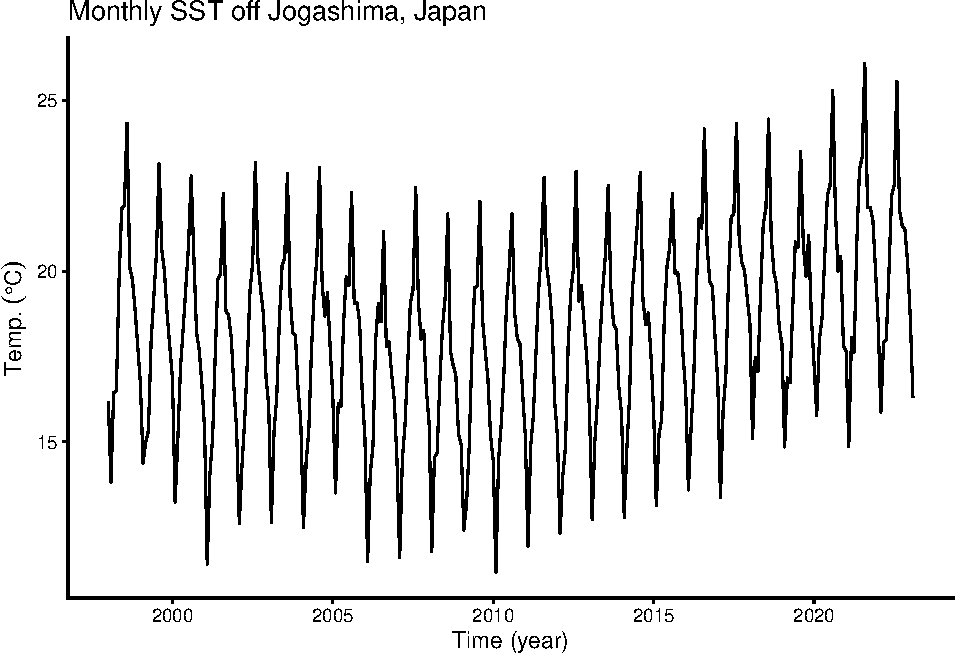
\includegraphics[keepaspectratio]{tempssm_manual_files/tempssm_manual_files/figure-latex/unnamed-chunk-3-1.pdf}}

The overall mean SST is approximately 18.2 °C, and a clear seasonal
pattern is visible. The series contains 0 missing observations. The raw
time series suggests that SST may have decreased gradually from the
beginning of the record to around 2008 and then increased thereafter.
However, interannual variability is also evident, making the long-term
pattern difficult to assess from the raw series alone.

\subsubsection{Applying a Linear Gaussian State-Space
Model}\label{applying-a-linear-gaussian-state-space-model}

When a \texttt{ts} object containing temperature time-series data (here,
\texttt{sst\_jogashima}) is passed to the core function
\texttt{tempssm()}, model construction and parameter estimation are
performed together. The returned S3 object of class \texttt{tempssm}
(here, \texttt{res\_ar1}) stores the filtering and smoothing estimates,
as well as the constructed model and input data. By default,
\texttt{tempssm()} fits a first-order autoregressive model.

\begin{Shaded}
\begin{Highlighting}[]
\CommentTok{\# model with first{-}order autoregressive component}
\NormalTok{res\_ar1 }\OtherTok{\textless{}{-}} \FunctionTok{tempssm}\NormalTok{(sst\_jogashima) }\CommentTok{\# (ar\_order=1: default)}
\FunctionTok{summary}\NormalTok{(res\_ar1)}
\end{Highlighting}
\end{Shaded}

\begin{verbatim}
## tempssm summary
## -----------------
## Call:
## tempssm(temp_data = sst_jogashima)
## 
## Model fit:
##   Likelihood type: marginal 
##   Log-likelihood : -198.19 
##   k              : 5 
##   Diffuse states : 13 
##   Converged      : TRUE 
## 
## Variance parameters:
##   Observation (H): 0.07496416 
##   State (Q trend): 4.937122e-06 
##   State (Q season): 0.0001763538 
##   State (Q ar): 0.1202156 
## 
## Components of auto-regression:
##   Order of AR: 1 
##   Coefficient of AR1: 0.7579372
\end{verbatim}

From the summary output, confirm that the model has converged
(\texttt{Converged:\ TRUE}). The output also reports statistics such as
the number of parameters (\texttt{k}), the log-likelihood, the
likelihood type, and the number of diffuse initial states. The parameter
estimates include the observation error variance (\texttt{H}), the
process error variance of the long-term trend component
(\texttt{Q\ trend}), the process error variance of the seasonal
component (\texttt{Q\ season}), the process error variance of the
autoregressive component, and the first-order autoregressive coefficient
(\texttt{AR1}).

The log-likelihood and the associated number of estimated parameters can
also be extracted directly from the fitted \texttt{tempssm} object using
\texttt{logLik()}.

\begin{Shaded}
\begin{Highlighting}[]
\NormalTok{ll }\OtherTok{\textless{}{-}} \FunctionTok{logLik}\NormalTok{(res\_ar1)}
\NormalTok{ll}
\end{Highlighting}
\end{Shaded}

\begin{verbatim}
## 'log Lik.' -198.1929 (df=5)
\end{verbatim}

\begin{Shaded}
\begin{Highlighting}[]
\FunctionTok{attr}\NormalTok{(ll, }\StringTok{"df"}\NormalTok{) }\CommentTok{\# number of parameters}
\end{Highlighting}
\end{Shaded}

\begin{verbatim}
## [1] 5
\end{verbatim}

By default, \texttt{tempssm()} uses the KFAS marginal likelihood for
parameter estimation. The diffuse likelihood remains available by
explicitly setting \texttt{marginal\ =\ FALSE}. The selected likelihood
type is stored in the fitted \texttt{tempssm} object and is used
consistently by downstream methods such as \texttt{logLik()} and
\texttt{summary()}.

The package intentionally does not compute AIC for \texttt{tempssm}
objects. This is because AIC comparisons for state-space models can
require care when likelihood type, diffuse initialization, or
latent-state structure differs across models. To avoid presenting AIC as
a default model-selection criterion, \texttt{tempssm} does not provide
automatic AIC-based comparison. Instead, this manual emphasizes a
model-assessment workflow based on residual diagnostics and time-series
cross-validation. The log-likelihood and parameter count remain
available through \texttt{logLik()} for users who need them for their
own model-assessment workflows.

\subsubsection{Plotting Long-Term Trend, Drift, Seasonal, and
Autoregressive
Components}\label{plotting-long-term-trend-drift-seasonal-and-autoregressive-components}

We extract the corresponding latent components from the state-space
model and visualize the estimated long-term evolution of temperature
levels and their rate of change (drift). Plotting seasonal variation and
autoregressive dependence as well makes the underlying trend structure
easier to examine.

\begin{Shaded}
\begin{Highlighting}[]
\CommentTok{\# plot all components at once}
\FunctionTok{plot}\NormalTok{(res\_ar1)}
\end{Highlighting}
\end{Shaded}

\pandocbounded{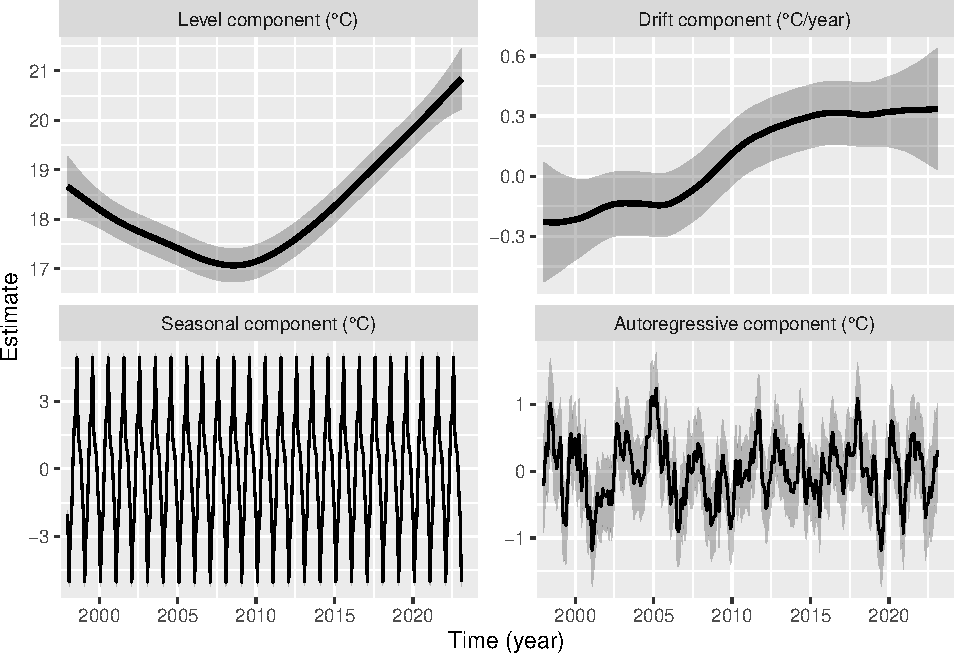
\includegraphics[keepaspectratio]{tempssm_manual_files/tempssm_manual_files/figure-latex/unnamed-chunk-7-1.pdf}}

The long-term trend in the upper-left panel suggests that SST decreased
during the first part of the study period and then increased after
around 2008. In this example, the average annual rate of SST change over
the full period is approximately 0.088 °C.

However, this full-period average should be interpreted together with
the time-varying drift component. In the upper-right panel, the drift
component is negative before around 2008 and becomes positive
thereafter, corresponding to the shift from a decreasing to an
increasing long-term SST pattern. The shaded gray areas represent 95\%
confidence intervals for the estimated latent states and illustrate the
uncertainty associated with each estimated component.

For scripted workflows, \texttt{plot\_tempssm\_components()} returns the
same component plot as a \texttt{ggplot} object;
\texttt{ggplot2::autoplot()} is also available. To obtain a ggplot
object for an individual component, specify the \texttt{component}
argument in \texttt{plot\_tempssm\_components()} as follows.

\begin{Shaded}
\begin{Highlighting}[]
\CommentTok{\# plot each of components at once}
\NormalTok{plt\_level }\OtherTok{\textless{}{-}} \FunctionTok{plot\_tempssm\_components}\NormalTok{(res\_ar1, }\AttributeTok{component =} \FunctionTok{c}\NormalTok{(}\StringTok{"level"}\NormalTok{))}
\NormalTok{plt\_drift }\OtherTok{\textless{}{-}} \FunctionTok{plot\_tempssm\_components}\NormalTok{(res\_ar1, }\AttributeTok{component =} \FunctionTok{c}\NormalTok{(}\StringTok{"drift"}\NormalTok{))}
\NormalTok{plt\_season }\OtherTok{\textless{}{-}} \FunctionTok{plot\_tempssm\_components}\NormalTok{(res\_ar1, }\AttributeTok{component =} \FunctionTok{c}\NormalTok{(}\StringTok{"season"}\NormalTok{))}
\NormalTok{plt\_ar }\OtherTok{\textless{}{-}} \FunctionTok{plot\_tempssm\_components}\NormalTok{(res\_ar1, }\AttributeTok{component =} \FunctionTok{c}\NormalTok{(}\StringTok{"ar"}\NormalTok{))}
\end{Highlighting}
\end{Shaded}

\subsubsection{Model Diagnostics}\label{model-diagnostics}

The package provides diagnostic tools for checking whether the fitted
model has left notable structure in the residuals. In particular,
residual time-series plots, residual autocorrelation, residual
distributions, and Ljung-Box tests can be used to assess remaining
temporal dependence and departures from the Gaussian error assumption.

\begin{Shaded}
\begin{Highlighting}[]
\NormalTok{r }\OtherTok{\textless{}{-}} \FunctionTok{get\_tempssm\_residuals}\NormalTok{(res\_ar1)}
\NormalTok{lb\_lag }\OtherTok{\textless{}{-}} \FunctionTok{frequency}\NormalTok{(res\_ar1}\SpecialCharTok{$}\NormalTok{temp\_data)}
\NormalTok{forecast}\SpecialCharTok{::}\FunctionTok{checkresiduals}\NormalTok{(r, }\AttributeTok{lag =}\NormalTok{ lb\_lag, }\AttributeTok{test =} \StringTok{"LB"}\NormalTok{)}
\end{Highlighting}
\end{Shaded}

\pandocbounded{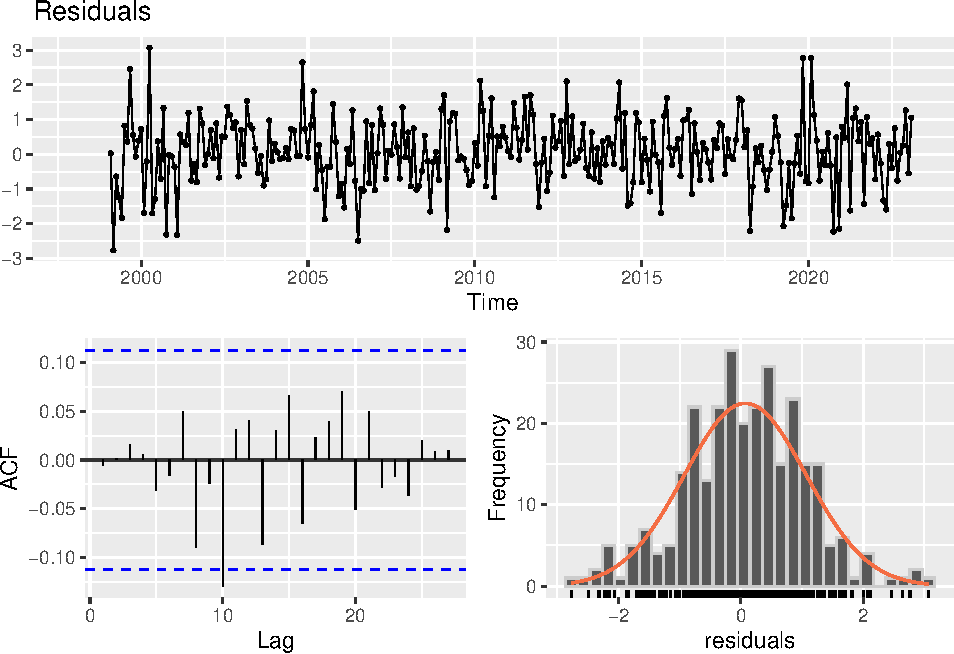
\includegraphics[keepaspectratio]{tempssm_manual_files/tempssm_manual_files/figure-latex/unnamed-chunk-10-1.pdf}}

\begin{verbatim}
## 
##  Ljung-Box test
## 
## data:  Residuals
## Q* = 9.6827, df = 12, p-value = 0.6438
## 
## Model df: 0.   Total lags used: 12
\end{verbatim}

Here, \texttt{get\_tempssm\_residuals()} extracts standardized recursive
residuals, and \texttt{forecast::checkresiduals()} displays their
time-series plot, ACF plot, histogram, and Ljung-Box test. The three
plots appear in the upper, lower-left, and lower-right panels,
respectively. The lag is set to the seasonal frequency of the input
data; for monthly data, this uses lag 12. These plots and the test
result should be checked for any notable residual patterns.

In this example, the ACF plot does not show a clear sequence of
successive significant lags or a repeated seasonal pattern. Isolated
spikes can occur when many lags are inspected, so they should be
interpreted together with the Ljung-Box test and the residual
time-series plot rather than used as the sole basis for changing the
model.

The package wrapper \texttt{plot\_tempssm\_residual\_diagnostics()} is
also available when a single function call for these diagnostic plots is
preferred.

For a compact tabular summary of the Ljung-Box test and residual
kurtosis, use \texttt{diagnose\_residuals()}.

\begin{Shaded}
\begin{Highlighting}[]
\NormalTok{diag }\OtherTok{\textless{}{-}} \FunctionTok{diagnose\_residuals}\NormalTok{(res\_ar1)}
\FunctionTok{print}\NormalTok{(diag)}
\end{Highlighting}
\end{Shaded}

\begin{verbatim}
## # A tibble: 1 x 4
##   lb_stat lb_lag lb_pvalue kurtosis
##     <dbl>  <dbl>     <dbl>    <dbl>
## 1    9.68     12     0.644     3.26
\end{verbatim}

The \texttt{lb\_stat}, \texttt{lb\_lag}, and \texttt{lb\_pvalue} columns
returned by \texttt{diagnose\_residuals()} correspond to the Ljung-Box
test statistic, the lag used in the test, and the corresponding P-value.
For monthly time series, the default Ljung-Box lag is the seasonal
frequency, so the default test evaluates residual autocorrelation up to
lag 12. In this example, the Ljung-Box test does not indicate
significant residual autocorrelation up to lag 12.

If residual autocorrelation at longer lags is of concern, the lag can be
specified manually. For example, the following code repeats the
Ljung-Box test up to lags 24 and 36.

\begin{Shaded}
\begin{Highlighting}[]
\NormalTok{diag\_lag24 }\OtherTok{\textless{}{-}} \FunctionTok{diagnose\_residuals}\NormalTok{(res\_ar1, }\AttributeTok{lb\_lag =} \DecValTok{24}\NormalTok{)}
\NormalTok{diag\_lag36 }\OtherTok{\textless{}{-}} \FunctionTok{diagnose\_residuals}\NormalTok{(res\_ar1, }\AttributeTok{lb\_lag =} \DecValTok{36}\NormalTok{)}

\NormalTok{diag\_lags }\OtherTok{\textless{}{-}} \FunctionTok{rbind}\NormalTok{(diag, diag\_lag24, diag\_lag36)}
\NormalTok{diag\_lags}\SpecialCharTok{$}\NormalTok{check }\OtherTok{\textless{}{-}} \FunctionTok{c}\NormalTok{(}\StringTok{"lag 12"}\NormalTok{, }\StringTok{"lag 24"}\NormalTok{, }\StringTok{"lag 36"}\NormalTok{)}
\NormalTok{diag\_lags[, }\FunctionTok{c}\NormalTok{(}\StringTok{"check"}\NormalTok{, }\StringTok{"lb\_stat"}\NormalTok{, }\StringTok{"lb\_lag"}\NormalTok{, }\StringTok{"lb\_pvalue"}\NormalTok{, }\StringTok{"kurtosis"}\NormalTok{)]}
\end{Highlighting}
\end{Shaded}

\begin{verbatim}
## # A tibble: 3 x 5
##   check  lb_stat lb_lag lb_pvalue kurtosis
##   <chr>    <dbl>  <dbl>     <dbl>    <dbl>
## 1 lag 12    9.68     12     0.644     3.26
## 2 lag 24   19.5      24     0.725     3.26
## 3 lag 36   27.9      36     0.831     3.26
\end{verbatim}

These diagnostics should be interpreted together with the residual ACF
plot. A small number of isolated ACF spikes can occur by chance when
many lags are inspected, whereas repeated or periodic spikes may suggest
remaining temporal structure.

\subsubsection{Examining the Autoregressive (AR)
Order}\label{examining-the-autoregressive-ar-order}

In this manual, the default AR(1) specification is used as the working
model. The autoregressive component is included to absorb short-term
serial dependence that is not represented by the latent level, drift,
and seasonal components. A higher AR order should therefore not be
treated as an automatic improvement. Instead, the AR order can be
adjusted when residual diagnostics suggest that notable autocorrelation
remains.

For example, if residual autocorrelation remains after fitting the AR(1)
model, users can fit an AR(2) model and repeat the same diagnostics.

\begin{Shaded}
\begin{Highlighting}[]
\CommentTok{\# Optional sensitivity check with a second{-}order autoregressive component}
\NormalTok{res\_ar2 }\OtherTok{\textless{}{-}} \FunctionTok{tempssm}\NormalTok{(sst\_jogashima, }\AttributeTok{ar\_order =} \DecValTok{2}\NormalTok{)}
\FunctionTok{summary}\NormalTok{(res\_ar2)}
\end{Highlighting}
\end{Shaded}

\begin{verbatim}
## tempssm summary
## -----------------
## Call:
## tempssm(temp_data = sst_jogashima, ar_order = 2)
## 
## Model fit:
##   Likelihood type: marginal 
##   Log-likelihood : -198.19 
##   k              : 6 
##   Diffuse states : 13 
##   Converged      : TRUE 
## 
## Variance parameters:
##   Observation (H): 0.05517452 
##   State (Q trend): 4.945287e-06 
##   State (Q season): 0.0001859987 
##   State (Q ar): 0.149755 
## 
## Components of auto-regression:
##   Order of AR: 2 
##   Coefficient of AR1: 0.6553237 
##   Coefficient of AR2: 0.07430046
\end{verbatim}

\begin{Shaded}
\begin{Highlighting}[]
\FunctionTok{plot\_tempssm\_residual\_diagnostics}\NormalTok{(res\_ar2)}
\end{Highlighting}
\end{Shaded}

\pandocbounded{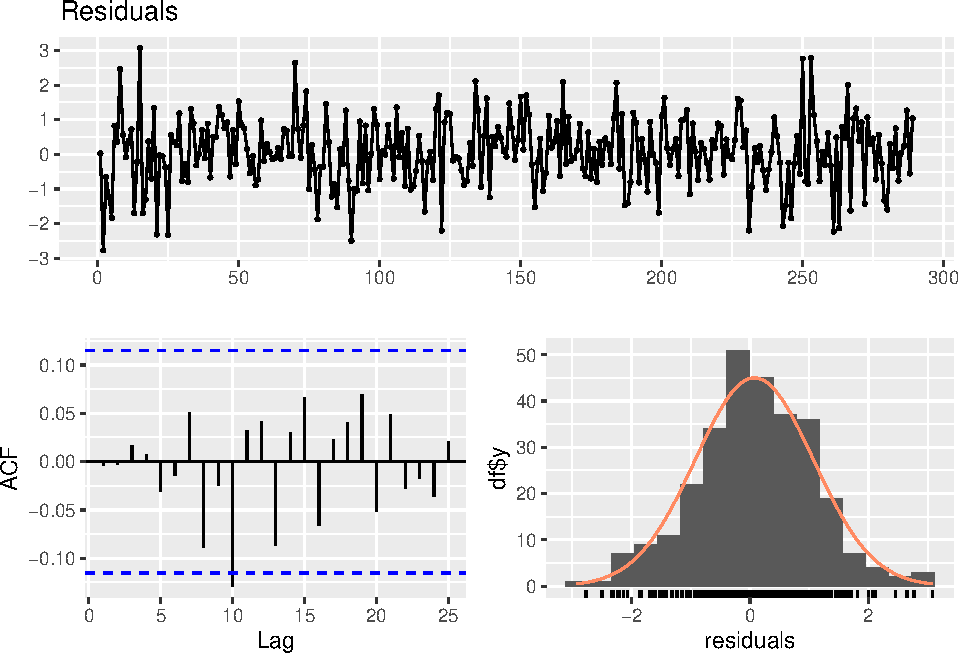
\includegraphics[keepaspectratio]{tempssm_manual_files/tempssm_manual_files/figure-latex/unnamed-chunk-13-1.pdf}}

\begin{Shaded}
\begin{Highlighting}[]
\NormalTok{diag\_lag12\_ar2 }\OtherTok{\textless{}{-}} \FunctionTok{diagnose\_residuals}\NormalTok{(res\_ar2, }\AttributeTok{lb\_lag =} \DecValTok{12}\NormalTok{)}
\NormalTok{diag\_lag24\_ar2 }\OtherTok{\textless{}{-}} \FunctionTok{diagnose\_residuals}\NormalTok{(res\_ar2, }\AttributeTok{lb\_lag =} \DecValTok{24}\NormalTok{)}
\NormalTok{diag\_lag36\_ar2 }\OtherTok{\textless{}{-}} \FunctionTok{diagnose\_residuals}\NormalTok{(res\_ar2, }\AttributeTok{lb\_lag =} \DecValTok{36}\NormalTok{)}
\NormalTok{diag\_lags\_ar2 }\OtherTok{\textless{}{-}} \FunctionTok{rbind}\NormalTok{(diag\_lag12\_ar2, diag\_lag24\_ar2, diag\_lag36\_ar2)}
\NormalTok{diag\_lags\_ar2}\SpecialCharTok{$}\NormalTok{check }\OtherTok{\textless{}{-}} \FunctionTok{c}\NormalTok{(}\StringTok{"lag 12"}\NormalTok{, }\StringTok{"lag 24"}\NormalTok{, }\StringTok{"lag 36"}\NormalTok{)}
\NormalTok{diag\_lags\_ar2[, }\FunctionTok{c}\NormalTok{(}\StringTok{"check"}\NormalTok{, }\StringTok{"lb\_stat"}\NormalTok{, }\StringTok{"lb\_lag"}\NormalTok{, }\StringTok{"lb\_pvalue"}\NormalTok{, }\StringTok{"kurtosis"}\NormalTok{)]}
\end{Highlighting}
\end{Shaded}

\begin{verbatim}
## # A tibble: 3 x 5
##   check  lb_stat lb_lag lb_pvalue kurtosis
##   <chr>    <dbl>  <dbl>     <dbl>    <dbl>
## 1 lag 12    9.61     12     0.650     3.26
## 2 lag 24   19.4      24     0.729     3.26
## 3 lag 36   27.9      36     0.831     3.26
\end{verbatim}

In a sensitivity check with an AR(2) specification, the residual
diagnostics were very similar to those from the AR(1) model. This
suggests that increasing the AR order does not provide an obvious
diagnostic improvement in this example.

In the present example, the residual diagnostics do not provide strong
evidence that a higher AR order is needed, so we proceed with the AR(1)
model as the baseline specification.

\subsubsection{Estimated Parameters and Latent-State
Components}\label{estimated-parameters-and-latent-state-components}

The fitted \texttt{tempssm} object contains the smoothed state estimates
returned by \texttt{KFAS}. The matrix \texttt{res\_ar1\$kfs\$alphahat}
stores these latent-state estimates, including the level, drift,
seasonal states, and autoregressive state. Inspecting this matrix is
useful for understanding the internal state representation.

\begin{Shaded}
\begin{Highlighting}[]
\CommentTok{\# Smoothing estimates}
\NormalTok{alpha\_hat }\OtherTok{\textless{}{-}}\NormalTok{ res\_ar1}\SpecialCharTok{$}\NormalTok{kfs}\SpecialCharTok{$}\NormalTok{alphahat}
\FunctionTok{head}\NormalTok{(alpha\_hat)}
\end{Highlighting}
\end{Shaded}

\begin{verbatim}
##             level       slope sea_dummy1 sea_dummy2 sea_dummy3 sea_dummy4
## Jan 1998 18.65840 -0.01905354 -2.0428374 -0.9196344  0.5642451  0.9553992
## Feb 1998 18.63934 -0.01906722 -5.0256252 -2.0428374 -0.9196344  0.5642451
## Mar 1998 18.62028 -0.01909100 -2.8244535 -5.0256252 -2.0428374 -0.9196344
## Apr 1998 18.60118 -0.01911003 -2.0508949 -2.8244535 -5.0256252 -2.0428374
## May 1998 18.58207 -0.01914415  0.2882283 -2.0508949 -2.8244535 -5.0256252
## Jun 1998 18.56293 -0.01918604  1.9925949  0.2882283 -2.0508949 -2.8244535
##          sea_dummy5 sea_dummy6 sea_dummy7 sea_dummy8 sea_dummy9 sea_dummy10
## Jan 1998  1.6282639  4.9410126  2.4937014  1.9925949  0.2882283  -2.0508949
## Feb 1998  0.9553992  1.6282639  4.9410126  2.4937014  1.9925949   0.2882283
## Mar 1998  0.5642451  0.9553992  1.6282639  4.9410126  2.4937014   1.9925949
## Apr 1998 -0.9196344  0.5642451  0.9553992  1.6282639  4.9410126   2.4937014
## May 1998 -2.0428374 -0.9196344  0.5642451  0.9553992  1.6282639   4.9410126
## Jun 1998 -5.0256252 -2.0428374 -0.9196344  0.5642451  0.9553992   1.6282639
##          sea_dummy11     arima1
## Jan 1998  -2.8244535 -0.2178662
## Feb 1998  -2.0508949  0.1519895
## Mar 1998   0.2882283  0.4187224
## Apr 1998   1.9925949  0.2408084
## May 1998   2.4937014  0.7185730
## Jun 1998   4.9410126  1.0167731
\end{verbatim}

For routine use, helper functions provide a simpler way to extract
individual components as \texttt{ts} objects with the original time
index. The level component represents the estimated long-term
temperature level, while the drift component represents its rate of
change per year.

\begin{Shaded}
\begin{Highlighting}[]
\CommentTok{\# Smoothing estimate of level component}
\NormalTok{level\_ts }\OtherTok{\textless{}{-}} \FunctionTok{get\_level\_ts}\NormalTok{(res\_ar1)}

\CommentTok{\# Smoothing estimate of drift component}
\NormalTok{drift\_ts }\OtherTok{\textless{}{-}} \FunctionTok{get\_drift\_ts}\NormalTok{(res\_ar1)}

\CommentTok{\# Average drift rate per year across the full period}
\NormalTok{mean\_drift\_year }\OtherTok{\textless{}{-}} \FunctionTok{mean}\NormalTok{(drift\_ts) }
\FunctionTok{print}\NormalTok{(mean\_drift\_year)}
\end{Highlighting}
\end{Shaded}

\begin{verbatim}
## [1] 0.08777084
\end{verbatim}

The average annual rate of SST change was estimated to be 0.0878 °C over
the full period. Because the estimated drift changes sign over time,
this value should be interpreted as a model-based summary of the whole
study period rather than as a constant warming rate.

\subsubsection{Short-Term Prediction}\label{short-term-prediction}

A fitted \texttt{tempssm} object can also be passed to
\texttt{predict()} to obtain short-term predictions. By default,
\texttt{predict(res)} returns a one-step-ahead prediction beyond the end
of the observed series. This is useful for visual checks of how the
fitted model extrapolates the estimated level, seasonal, and
autoregressive components.

\begin{Shaded}
\begin{Highlighting}[]
\NormalTok{pred\_1 }\OtherTok{\textless{}{-}} \FunctionTok{predict}\NormalTok{(res\_ar1)}
\NormalTok{pred\_1}
\end{Highlighting}
\end{Shaded}

\begin{verbatim}
##           Mar
## 2023 18.33035
\end{verbatim}

Predictions for multiple future time points can be requested by setting
the \texttt{n.ahead} argument.

\begin{Shaded}
\begin{Highlighting}[]
\NormalTok{pred\_12 }\OtherTok{\textless{}{-}} \FunctionTok{predict}\NormalTok{(res\_ar1, }\AttributeTok{n.ahead =} \DecValTok{12}\NormalTok{)}
\NormalTok{pred\_12}
\end{Highlighting}
\end{Shaded}

\begin{verbatim}
##           Jan      Feb      Mar      Apr      May      Jun      Jul      Aug
## 2023                   18.33035 18.96985 21.33710 23.08522 23.51856 26.03694
## 2024 19.09319 16.16926                                                      
##           Sep      Oct      Nov      Dec
## 2023 22.69098 22.00902 21.74806 20.19190
## 2024
\end{verbatim}

Prediction uncertainty can also be returned by setting the
\texttt{interval} argument. With \texttt{interval\ =\ "confidence"}, the
returned lower and upper bounds describe uncertainty in the predicted
mean response. With \texttt{interval\ =\ "prediction"}, the bounds
describe uncertainty in a future observation and therefore also include
observation error; prediction intervals are usually wider than
confidence intervals. The confidence level is controlled by the
\texttt{level} argument and defaults to 0.95.

\begin{Shaded}
\begin{Highlighting}[]
\NormalTok{pred\_12\_pi }\OtherTok{\textless{}{-}} \FunctionTok{predict}\NormalTok{(}
\NormalTok{  res\_ar1,}
  \AttributeTok{n.ahead =} \DecValTok{12}\NormalTok{,}
  \AttributeTok{interval =} \StringTok{"prediction"}\NormalTok{,}
  \AttributeTok{level =} \FloatTok{0.95}
\NormalTok{)}

\NormalTok{pred\_12\_pi}
\end{Highlighting}
\end{Shaded}

\begin{verbatim}
##               fit      lwr      upr
## Mar 2023 18.33035 17.35029 19.31042
## Apr 2023 18.96985 17.85360 20.08610
## May 2023 21.33710 20.13453 22.53967
## Jun 2023 23.08522 21.82425 24.34619
## Jul 2023 23.51856 22.21551 24.82161
## Aug 2023 26.03694 24.70183 27.37204
## Sep 2023 22.69098 21.33016 24.05179
## Oct 2023 22.00902 20.62664 23.39141
## Nov 2023 21.74806 20.34682 23.14929
## Dec 2023 20.19190 18.77359 21.61020
## Jan 2024 19.09319 17.65904 20.52734
## Feb 2024 16.16926 14.72135 17.61717
\end{verbatim}

These predictions should be interpreted as model-based extrapolations
rather than definitive forecasts. Uncertainty generally increases as the
prediction horizon becomes longer, and long-horizon predictions can be
sensitive to model assumptions about trend, seasonality, and
autoregressive dependence.

\subsection{Exercise II: Applying a State-Space Model to a Temperature
Time Series with an Exogenous
Variable}\label{exercise-ii-applying-a-state-space-model-to-a-temperature-time-series-with-an-exogenous-variable}

\subsubsection{Objective}\label{objective-1}

We extend the state-space modeling framework to examine the effect of an
exogenous factor on temperature variation. Specifically, we examine the
effect of the Pacific Decadal Oscillation (PDO) as an exogenous variable
on SST observed off Yamaguchi Prefecture, Japan.

\subsubsection{Loading the PDO Index Dataset: PDO Index as an Exogenous
Variable}\label{loading-the-pdo-index-dataset-pdo-index-as-an-exogenous-variable}

\begin{itemize}
\tightlist
\item
  \textbf{Data}: Monthly Pacific Decadal Oscillation (PDO) index (JMA)\\
\item
  \textbf{Period}: January 1901 to December 2025
\end{itemize}

The Pacific Decadal Oscillation (PDO) index is defined as the projection
of monthly mean sea surface temperature (SST) anomalies onto the leading
empirical orthogonal function (EOF) of SST variability over the North
Pacific north of 20°N. The EOF is computed using SST anomalies for
1901--2000, defined relative to the 1901--2000 monthly climatology. To
remove the global warming signal, the global-mean SST anomaly is
subtracted from each grid point prior to the EOF analysis. In this
package, we use the PDO index provided by the Japan Meteorological
Agency (JMA), available at
\url{https://www.data.jma.go.jp/kaiyou/data/shindan/b_1/pdo/pdo.txt}.

\begin{Shaded}
\begin{Highlighting}[]
\FunctionTok{data}\NormalTok{(pdo) }\CommentTok{\# load a ts object of PDO index}
\FunctionTok{head}\NormalTok{(pdo)}
\end{Highlighting}
\end{Shaded}

\begin{verbatim}
##          Jan     Feb     Mar     Apr     May     Jun
## 1901  1.0040  0.7403  0.9011 -0.0109 -0.2325 -0.6810
\end{verbatim}

\subsubsection{Intersecting the Temperature and PDO Time
Series}\label{intersecting-the-temperature-and-pdo-time-series}

For state-space modeling with exogenous variables, all input time series
must share a common and aligned time index. In this step, the
temperature and PDO time series are restricted to their overlapping
period by trimming the leading and trailing portions so that both
datasets cover the same time span.

The function \texttt{tempssm::trim\_ts\_overlap()} is used to align the
two \texttt{ts} objects on a shared timeline and returns time series
containing only the common period.

\begin{Shaded}
\begin{Highlighting}[]
\CommentTok{\# Generate an object on a shared timeline}
\NormalTok{trimmed\_series }\OtherTok{\textless{}{-}} \FunctionTok{trim\_ts\_overlap}\NormalTok{(yamaguchi\_sst,}
\NormalTok{                                  pdo,}
                                  \AttributeTok{temp\_name =} \StringTok{"Temp"}\NormalTok{,}
                                  \AttributeTok{exo\_name =} \StringTok{"PDO"}\NormalTok{)}

\NormalTok{yamaguchi\_sst\_trim }\OtherTok{\textless{}{-}}\NormalTok{ trimmed\_series}\SpecialCharTok{$}\NormalTok{temperature}
\NormalTok{pdo\_trim }\OtherTok{\textless{}{-}}\NormalTok{ trimmed\_series}\SpecialCharTok{$}\NormalTok{exogenous}

\FunctionTok{start}\NormalTok{(yamaguchi\_sst\_trim)}
\end{Highlighting}
\end{Shaded}

\begin{verbatim}
## [1] 1982    1
\end{verbatim}

\begin{Shaded}
\begin{Highlighting}[]
\FunctionTok{end}\NormalTok{(yamaguchi\_sst\_trim)}
\end{Highlighting}
\end{Shaded}

\begin{verbatim}
## [1] 2025   12
\end{verbatim}

\begin{Shaded}
\begin{Highlighting}[]
\FunctionTok{start}\NormalTok{(pdo\_trim)}
\end{Highlighting}
\end{Shaded}

\begin{verbatim}
## [1] 1982    1
\end{verbatim}

\begin{Shaded}
\begin{Highlighting}[]
\FunctionTok{end}\NormalTok{(pdo\_trim)}
\end{Highlighting}
\end{Shaded}

\begin{verbatim}
## [1] 2025   12
\end{verbatim}

\subsubsection{Plotting Time Series of SST and the PDO
Index}\label{plotting-time-series-of-sst-and-the-pdo-index}

We visualize the time-series structures of SST and the PDO index.

\begin{Shaded}
\begin{Highlighting}[]
\NormalTok{plt\_yamaguchi\_sst\_trim }\OtherTok{\textless{}{-}}\NormalTok{ forecast}\SpecialCharTok{::}\FunctionTok{autoplot}\NormalTok{(yamaguchi\_sst\_trim) }\SpecialCharTok{+}
  \FunctionTok{labs}\NormalTok{(}\AttributeTok{y =} \FunctionTok{expression}\NormalTok{(Temp.}\SpecialCharTok{\textasciitilde{}}\NormalTok{(degree}\SpecialCharTok{*}\NormalTok{C)), }
       \AttributeTok{x =} \StringTok{"Time (year)"}\NormalTok{) }\SpecialCharTok{+}
  \FunctionTok{ggtitle}\NormalTok{(}\StringTok{"Monthly SST off Yamaguchi, Japan"}\NormalTok{) }\SpecialCharTok{+}
  \FunctionTok{theme\_classic}\NormalTok{()}


\NormalTok{plt\_pdo }\OtherTok{\textless{}{-}}\NormalTok{ forecast}\SpecialCharTok{::}\FunctionTok{autoplot}\NormalTok{(pdo\_trim) }\SpecialCharTok{+}
  \FunctionTok{labs}\NormalTok{(}\AttributeTok{x =} \StringTok{"Time (year)"}\NormalTok{, }\AttributeTok{y =} \StringTok{"PDO index"}\NormalTok{) }\SpecialCharTok{+}
  \FunctionTok{ggtitle}\NormalTok{(}\StringTok{"PDO index"}\NormalTok{) }\SpecialCharTok{+}
  \FunctionTok{theme\_classic}\NormalTok{()}

\NormalTok{plt\_yamaguchi\_sst\_trim }\SpecialCharTok{+}\NormalTok{ plt\_pdo }\SpecialCharTok{+}\NormalTok{ patchwork}\SpecialCharTok{::}\FunctionTok{plot\_layout}\NormalTok{(}\AttributeTok{ncol=}\DecValTok{1}\NormalTok{)}
\end{Highlighting}
\end{Shaded}

\pandocbounded{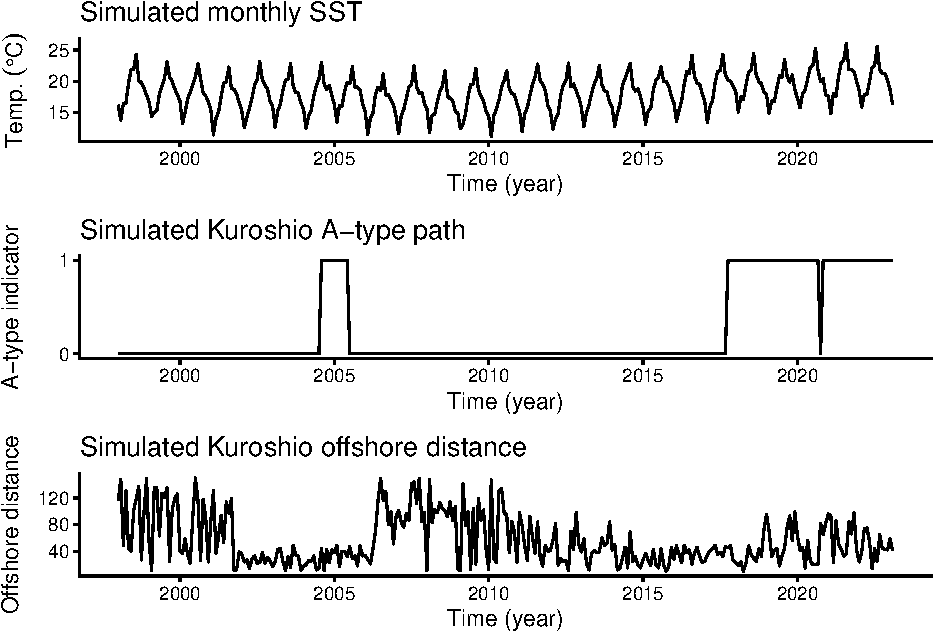
\includegraphics[keepaspectratio]{tempssm_manual_files/tempssm_manual_files/figure-latex/unnamed-chunk-21-1.pdf}}

The PDO index data used in this exercise contain no missing values. When
using your own exogenous-variable data, however, make sure that the
exogenous variables do not contain missing values before fitting the
model. \texttt{tempssm()} does not allow missing values in exogenous
variables, and model fitting will stop with an error if such data are
supplied. If necessary, apply appropriate preprocessing, such as
imputation, before the analysis.

In contrast, missing values in the dependent temperature time series are
allowed. In the state-space model, these missing values are treated as
unobserved responses, and model estimation proceeds through Kalman
filtering and smoothing.

\subsubsection{Applying a Model Without an Exogenous
Variable}\label{applying-a-model-without-an-exogenous-variable}

We first apply a baseline state-space model that does not include any
exogenous variables. This model serves as a reference case in which
temperature variation is explained solely by the latent long-term trend,
seasonal cycle, and autoregressive dependence. Although the same model
was already fitted in Exercise I, here we explicitly specify the
dependent-variable argument and store the returned object as
\texttt{res\_without}.

\begin{Shaded}
\begin{Highlighting}[]
\NormalTok{res\_without }\OtherTok{\textless{}{-}} \FunctionTok{tempssm}\NormalTok{(}\AttributeTok{temp\_data =}\NormalTok{ yamaguchi\_sst\_trim, }\AttributeTok{ar\_order =} \DecValTok{1}\NormalTok{) }
\FunctionTok{summary}\NormalTok{(res\_without)}
\end{Highlighting}
\end{Shaded}

\begin{verbatim}
## tempssm summary
## -----------------
## Call:
## tempssm(temp_data = yamaguchi_sst_trim, ar_order = 1)
## 
## Model fit:
##   Likelihood type: marginal 
##   Log-likelihood : -435.46 
##   k              : 5 
##   Diffuse states : 13 
##   Converged      : TRUE 
## 
## Variance parameters:
##   Observation (H): 2.019273e-14 
##   State (Q trend): 1.118445e-07 
##   State (Q season): 2.312771e-149 
##   State (Q ar): 0.3164652 
## 
## Components of auto-regression:
##   Order of AR: 1 
##   Coefficient of AR1: 0.6205502
\end{verbatim}

\begin{Shaded}
\begin{Highlighting}[]
\FunctionTok{plot\_tempssm\_residual\_diagnostics}\NormalTok{(res\_without)}
\end{Highlighting}
\end{Shaded}

\pandocbounded{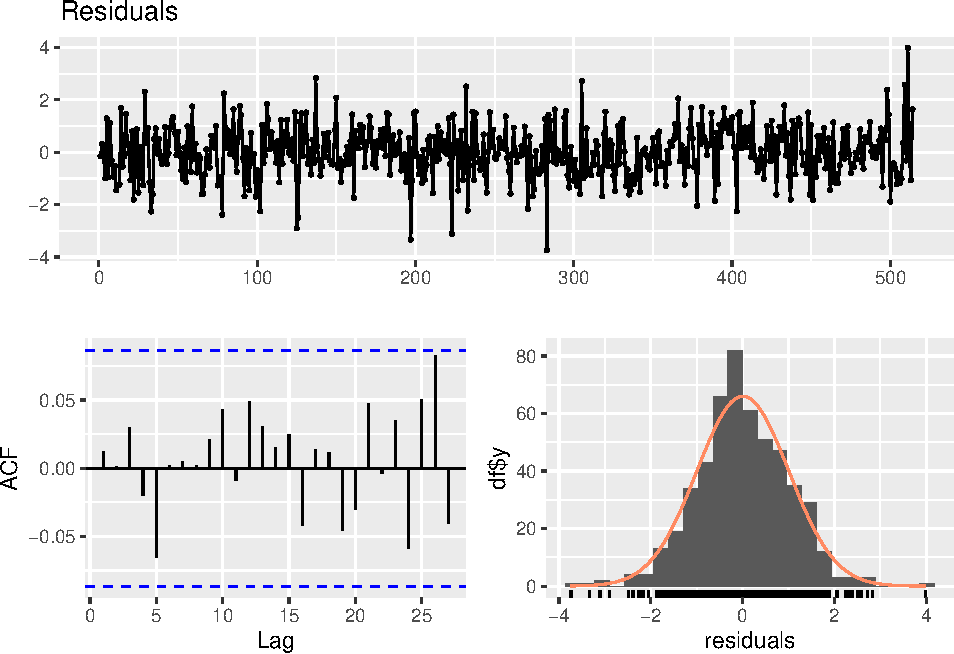
\includegraphics[keepaspectratio]{tempssm_manual_files/tempssm_manual_files/figure-latex/unnamed-chunk-22-1.pdf}}

\begin{Shaded}
\begin{Highlighting}[]
\NormalTok{diag\_res\_without }\OtherTok{\textless{}{-}} \FunctionTok{diagnose\_residuals}\NormalTok{(res\_without)}
\FunctionTok{print}\NormalTok{(diag\_res\_without)}
\end{Highlighting}
\end{Shaded}

\begin{verbatim}
## # A tibble: 1 x 4
##   lb_stat lb_lag lb_pvalue kurtosis
##     <dbl>  <dbl>     <dbl>    <dbl>
## 1    17.0     12     0.149     3.68
\end{verbatim}

The residual diagnostics for this AR(1) baseline model do not indicate
significant residual autocorrelation up to lag 12. This result suggests
that the default first-order autoregressive structure is a reasonable
starting point for the model without the exogenous variable.

This baseline model provides a useful benchmark for evaluating the
additional explanatory power of the PDO index introduced in the next
section.

\subsubsection{Applying a Model With an Exogenous
Variable}\label{applying-a-model-with-an-exogenous-variable}

We construct a model that uses the PDO index as a univariate exogenous
variable. In the \texttt{tempssm()} function, the PDO data
(\texttt{pdo\_trim}) are supplied to the exogenous-variable argument
(\texttt{exo\_data}). The temperature time series
(\texttt{yamaguchi\_sst\_trim}) is supplied to the dependent-variable
argument (\texttt{temp\_data}), which was implicit in the previous
examples.

\begin{Shaded}
\begin{Highlighting}[]
\NormalTok{res\_with }\OtherTok{\textless{}{-}} \FunctionTok{tempssm}\NormalTok{(}\AttributeTok{temp\_data =}\NormalTok{ yamaguchi\_sst\_trim,}
                    \AttributeTok{exo\_data =}\NormalTok{ pdo\_trim,}
                    \AttributeTok{ar\_order =} \DecValTok{1}\NormalTok{) }
\FunctionTok{summary}\NormalTok{(res\_with)}
\end{Highlighting}
\end{Shaded}

\begin{verbatim}
## tempssm summary
## -----------------
## Call:
## tempssm(temp_data = yamaguchi_sst_trim, exo_data = pdo_trim, 
##     ar_order = 1)
## 
## Model fit:
##   Likelihood type: marginal 
##   Log-likelihood : -390.99 
##   k              : 6 
##   Diffuse states : 14 
##   Converged      : TRUE 
## 
## Variance parameters:
##   Observation (H): 1.490122e-25 
##   State (Q trend): 7.158619e-20 
##   State (Q season): 2.316533e-82 
##   State (Q ar): 0.2695508 
## 
## Components of auto-regression:
##   Order of AR: 1 
##   Coefficient of AR1: 0.6566528 
## Exogenous variable    PDO 
## Estimated coefficient     -0.4476073 
## Lower CI  -0.5372882 
## Upper CI  -0.3579264
\end{verbatim}

\begin{Shaded}
\begin{Highlighting}[]
\FunctionTok{plot\_tempssm\_residual\_diagnostics}\NormalTok{(res\_with)}
\end{Highlighting}
\end{Shaded}

\pandocbounded{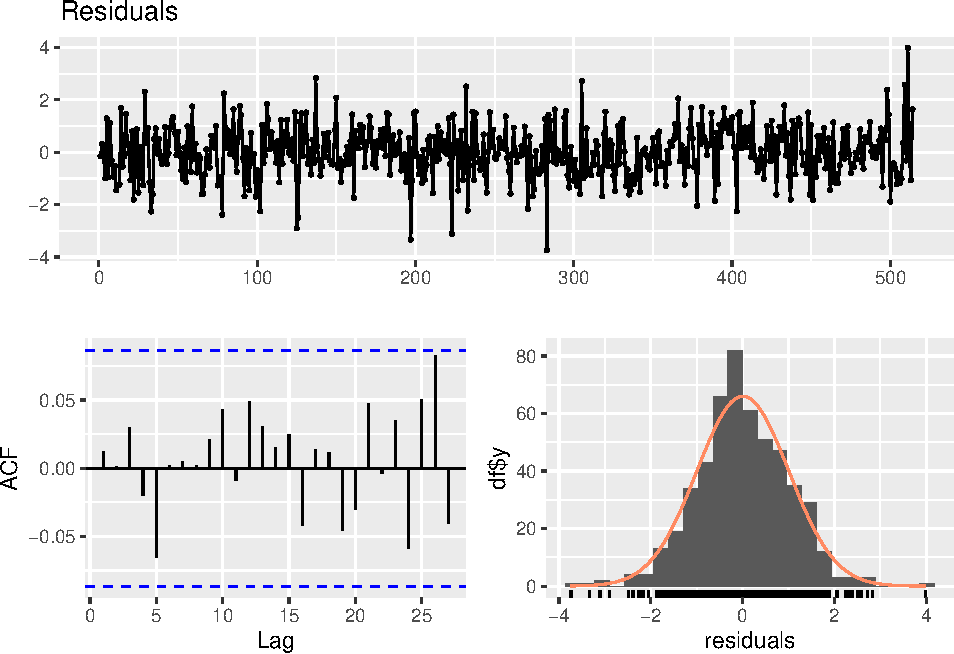
\includegraphics[keepaspectratio]{tempssm_manual_files/tempssm_manual_files/figure-latex/unnamed-chunk-23-1.pdf}}

\begin{Shaded}
\begin{Highlighting}[]
\NormalTok{diag\_res\_with }\OtherTok{\textless{}{-}} \FunctionTok{diagnose\_residuals}\NormalTok{(res\_with)}
\FunctionTok{print}\NormalTok{(diag\_res\_with)}
\end{Highlighting}
\end{Shaded}

\begin{verbatim}
## # A tibble: 1 x 4
##   lb_stat lb_lag lb_pvalue kurtosis
##     <dbl>  <dbl>     <dbl>    <dbl>
## 1    5.53     12     0.938     3.69
\end{verbatim}

The residual diagnostics for the model with the PDO index also do not
indicate significant residual autocorrelation up to lag 12. Thus, for
both models considered here, the AR(1) specification provides an
adequate working autoregressive structure according to these residual
checks.

We then examine the model estimates. The estimated coefficient for the
exogenous PDO index is negative (-0.45), and its 95\% confidence
interval does not include zero, ranging from -0.54 to -0.36. This
indicates a statistically significant negative relationship between
local SST off Yamaguchi Prefecture and PDO variability.

Specifically, after accounting for the underlying long-term trend,
seasonal cycle, and autoregressive dependence, the model suggests that a
one-unit increase in the PDO index is associated with an average
decrease of approximately 0.45 °C in monthly SST. This result implies
that positive phases of the PDO systematically contribute to cooler
conditions at the study site.

Importantly, the effect of this exogenous variable is identified as an
additional factor beyond the internal dynamics of the temperature time
series, rather than as an artifact of improved representation of the
long-term trend or temporal dependence. Compared with the baseline model
without exogenous variables, the statistical significance of the PDO
coefficient indicates that the PDO acts as an independent large-scale
climate driver influencing local temperature variation.

For models with exogenous variables, future values of the exogenous
variables are needed when calling \texttt{predict()}. If such values are
available, they can be passed through \texttt{new\_exo\_data}. For a
simple one-step-ahead visual check, \texttt{exo\_strategy\ =\ "last"}
carries the final observed exogenous value forward. This is a
persistence assumption for the exogenous variable, not a separate
forecast model for the PDO index.

\begin{Shaded}
\begin{Highlighting}[]
\NormalTok{pred\_with\_last\_exo }\OtherTok{\textless{}{-}} \FunctionTok{predict}\NormalTok{(res\_with, }\AttributeTok{exo\_strategy =} \StringTok{"last"}\NormalTok{)}
\NormalTok{pred\_with\_last\_exo}
\end{Highlighting}
\end{Shaded}

\begin{verbatim}
##           Jan
## 2026 16.41488
\end{verbatim}

\subsubsection{Time-Series Cross-Validation
(tsCV)}\label{time-series-cross-validation-tscv}

Time-series cross-validation (tsCV) evaluates model performance based on
out-of-sample prediction errors while respecting the temporal ordering
of the data. It therefore provides an additional and independent
perspective on model adequacy.

In time-series cross-validation, the model is repeatedly fitted to
expanding or sliding training windows, and predictive performance is
evaluated on subsequent observations. Unlike random cross-validation,
this procedure prevents information leakage from the future to the past
and is therefore suitable for model validation with temporal data.

Here, by comparing cross-validation metrics for models with and without
the exogenous PDO variable, we assess whether the statistical signal
found in the PDO coefficient is also reflected in out-of-sample
predictive performance.

For the model with the PDO index, the test-period PDO values are
supplied to the forecast step as exogenous variables. Therefore, this
tsCV setting evaluates conditional forecasts, or hindcasts, under the
assumption that the PDO values during each test period are known. This
is appropriate when the aim is to assess the explanatory or
reconstructive value of the PDO index.

For real-time future forecasting, however, future PDO values are usually
unknown. In that setting, users must either provide future PDO
scenarios, forecast the PDO index with a separate model, or use a
simplified assumption such as carrying the last observed value forward.
The results below should therefore be interpreted as evidence for
improved conditional predictive performance, not as a direct guarantee
of operational forecast improvement.

\begin{Shaded}
\begin{Highlighting}[]
\CommentTok{\# (Optional) Load packages for parallel processing.}
\CommentTok{\# These are only required if you want to enable parallel execution:}
\CommentTok{\# {-} future: controls how parallel workers are launched}
\CommentTok{\# {-} future.apply: provides parallelized apply functions}
\CommentTok{\# {-} progressr: optional progress bar support}
\FunctionTok{library}\NormalTok{(future.apply)}
\FunctionTok{library}\NormalTok{(future)}
\FunctionTok{library}\NormalTok{(progressr)}

\ControlFlowTok{if}\NormalTok{ (}\FunctionTok{interactive}\NormalTok{()) \{}
\NormalTok{  future}\SpecialCharTok{::}\FunctionTok{plan}\NormalTok{(multisession)}
\NormalTok{\} }\ControlFlowTok{else}\NormalTok{ \{}
\NormalTok{  future}\SpecialCharTok{::}\FunctionTok{plan}\NormalTok{(sequential)}
\NormalTok{\}}


\CommentTok{\# ts cross{-}validation of the model without exogenous variables}

\DocumentationTok{\#\# Generate a list of training and test datasets with their indices}
\CommentTok{\# Procedure for constructing year{-}based time{-}series cross{-}validation folds:}
\CommentTok{\# }
\CommentTok{\# First training data: January 1982–December 2017;}
\CommentTok{\# First test data: one year starting from January 2018}
\CommentTok{\# }
\CommentTok{\# Second training data: January 1983–December 2018;}
\CommentTok{\# Second test data: one year starting from January 2019}
\CommentTok{\# ...}
\CommentTok{\# }
\CommentTok{\# Eighth training data: January 1989–December 2024;}
\CommentTok{\# Eighth test data: one year starting from January 2025}
\CommentTok{\#}
\CommentTok{\# These folds are automatically generated by the ts\_train\_test\_split() function.}

\CommentTok{\# Generate training and test dataset for model without PDO index}
\NormalTok{folds\_without }\OtherTok{\textless{}{-}} \FunctionTok{ts\_train\_test\_split}\NormalTok{(}
  \AttributeTok{temp\_data =}\NormalTok{ yamaguchi\_sst\_trim,}
  \AttributeTok{exo\_data =} \ConstantTok{NULL}\NormalTok{,}
  \AttributeTok{initial =} \DecValTok{432}\NormalTok{, }\CommentTok{\# 432 monthly observations from Jan 1982 to Dec 2017}
  \AttributeTok{horizon =} \DecValTok{12}\NormalTok{, }\CommentTok{\# forecast 12 monthly time{-}series}
  \AttributeTok{step =} \DecValTok{12}\NormalTok{, }\CommentTok{\# training data is moved in one{-}year steps}
  \AttributeTok{fixed\_window =} \ConstantTok{TRUE}\NormalTok{,}
  \AttributeTok{allow\_partial =} \ConstantTok{FALSE}
\NormalTok{  )}

\CommentTok{\# Generate training and test dataset for model with PDO index}
\NormalTok{folds\_with }\OtherTok{\textless{}{-}} \FunctionTok{ts\_train\_test\_split}\NormalTok{(}
  \AttributeTok{temp\_data =}\NormalTok{ yamaguchi\_sst\_trim,}
  \AttributeTok{exo\_data =}\NormalTok{ pdo\_trim,}
  \AttributeTok{initial =} \DecValTok{432}\NormalTok{, }\CommentTok{\# 432 monthly observations from Jan 1982 to Dec 2017}
  \AttributeTok{horizon =} \DecValTok{12}\NormalTok{, }\CommentTok{\# forecast 12 monthly time{-}series}
  \AttributeTok{step =} \DecValTok{12}\NormalTok{, }\CommentTok{\# training data is moved in one{-}year steps}
  \AttributeTok{fixed\_window =} \ConstantTok{TRUE}\NormalTok{,}
  \AttributeTok{allow\_partial =} \ConstantTok{FALSE}
\NormalTok{  )}


\CommentTok{\# *****************************************}
\CommentTok{\# Executing time{-}series cross validation}

\CommentTok{\#{-}{-}{-}{-}{-}{-}{-}{-}{-}{-}{-}{-}{-}{-}{-}{-}{-}{-}{-}{-}{-}{-}{-}{-}{-}{-}{-}{-}{-}{-}{-}{-}{-}{-}{-}{-}{-}{-}{-}{-}{-}{-}{-}{-}{-}{-}{-}{-}{-}{-} }
\CommentTok{\# Model without the exogenous variable of PDO index}

\CommentTok{\# Single processing}
\CommentTok{\# cv\_without\_results \textless{}{-} ts\_cv\_run(folds\_without, ar\_order = 1, use\_season = TRUE)}

\CommentTok{\# Parallel processing}
\NormalTok{cv\_without\_results }\OtherTok{\textless{}{-}}\NormalTok{ future.apply}\SpecialCharTok{::}\FunctionTok{future\_lapply}\NormalTok{(}
\NormalTok{  folds\_without,}
\NormalTok{  ts\_cv\_run\_fold,}
  \AttributeTok{ar\_order =} \DecValTok{1}\NormalTok{,}
  \AttributeTok{use\_season =} \ConstantTok{TRUE}\NormalTok{,}
  \AttributeTok{future.seed =} \ConstantTok{TRUE}
\NormalTok{)}

\CommentTok{\# Computing assessment indexes}
\NormalTok{metrics\_without }\OtherTok{\textless{}{-}} \FunctionTok{lapply}\NormalTok{(cv\_without\_results, compute\_cv\_metrics)}

\CommentTok{\# tidy summary}
\NormalTok{cv\_without\_tbl }\OtherTok{\textless{}{-}} \FunctionTok{ts\_cv\_collect}\NormalTok{(cv\_without\_results, metrics\_without) }\SpecialCharTok{\%\textgreater{}\%}
  \FunctionTok{mutate}\NormalTok{(}\AttributeTok{Model=}\StringTok{"Without"}\NormalTok{)}


\CommentTok{\#{-}{-}{-}{-}{-}{-}{-}{-}{-}{-}{-}{-}{-}{-}{-}{-}{-}{-}{-}{-}{-}{-}{-}{-}{-}{-}{-}{-}{-}{-}{-}{-}{-}{-}{-}{-}{-}{-}{-}{-}{-}{-}{-}{-}{-}{-}{-}{-}{-}{-} }
\CommentTok{\# Model with the exogenous variable of PDO index}

\CommentTok{\# Single processing}
\CommentTok{\# cv\_with\_results \textless{}{-} ts\_cv\_run(folds\_with, ar\_order = 1, use\_season = TRUE)}

\CommentTok{\# Parallel processing}
\NormalTok{cv\_with\_results }\OtherTok{\textless{}{-}}\NormalTok{ future.apply}\SpecialCharTok{::}\FunctionTok{future\_lapply}\NormalTok{(}
\NormalTok{  folds\_with,}
\NormalTok{  ts\_cv\_run\_fold,}
  \AttributeTok{ar\_order =} \DecValTok{1}\NormalTok{,}
  \AttributeTok{use\_season =} \ConstantTok{TRUE}\NormalTok{,}
  \AttributeTok{future.seed =} \ConstantTok{TRUE}
\NormalTok{)}

\CommentTok{\# Computing assessment indexes}
\NormalTok{metrics\_with }\OtherTok{\textless{}{-}} \FunctionTok{lapply}\NormalTok{(cv\_with\_results, compute\_cv\_metrics)}

\CommentTok{\# tidy summary}
\NormalTok{cv\_with\_tbl }\OtherTok{\textless{}{-}} \FunctionTok{ts\_cv\_collect}\NormalTok{(cv\_with\_results, metrics\_with) }\SpecialCharTok{\%\textgreater{}\%}
  \FunctionTok{mutate}\NormalTok{(}\AttributeTok{Model=}\StringTok{"With"}\NormalTok{)}


\NormalTok{cv\_tbl }\OtherTok{\textless{}{-}} \FunctionTok{bind\_rows}\NormalTok{(cv\_without\_tbl, cv\_with\_tbl)}

\NormalTok{cv\_comparison }\OtherTok{\textless{}{-}} \FunctionTok{compare\_ts\_cv}\NormalTok{(}
  \FunctionTok{list}\NormalTok{(}
    \AttributeTok{Without =}\NormalTok{ cv\_without\_tbl,}
    \AttributeTok{With =}\NormalTok{ cv\_with\_tbl}
\NormalTok{  )}
\NormalTok{)}

\NormalTok{cv\_comparison }\SpecialCharTok{\%\textgreater{}\%}\NormalTok{ knitr}\SpecialCharTok{::}\FunctionTok{kable}\NormalTok{()}
\end{Highlighting}
\end{Shaded}

{\def\LTcaptype{none} % do not increment counter
\begin{longtable}[]{@{}
  >{\raggedright\arraybackslash}p{(\linewidth - 12\tabcolsep) * \real{0.0909}}
  >{\raggedleft\arraybackslash}p{(\linewidth - 12\tabcolsep) * \real{0.0909}}
  >{\raggedleft\arraybackslash}p{(\linewidth - 12\tabcolsep) * \real{0.1364}}
  >{\raggedleft\arraybackslash}p{(\linewidth - 12\tabcolsep) * \real{0.1705}}
  >{\raggedleft\arraybackslash}p{(\linewidth - 12\tabcolsep) * \real{0.1136}}
  >{\raggedleft\arraybackslash}p{(\linewidth - 12\tabcolsep) * \real{0.1818}}
  >{\raggedleft\arraybackslash}p{(\linewidth - 12\tabcolsep) * \real{0.2159}}@{}}
\toprule\noalign{}
\begin{minipage}[b]{\linewidth}\raggedright
model
\end{minipage} & \begin{minipage}[b]{\linewidth}\raggedleft
n\_folds
\end{minipage} & \begin{minipage}[b]{\linewidth}\raggedleft
converged\_n
\end{minipage} & \begin{minipage}[b]{\linewidth}\raggedleft
converged\_rate
\end{minipage} & \begin{minipage}[b]{\linewidth}\raggedleft
mean\_MAE
\end{minipage} & \begin{minipage}[b]{\linewidth}\raggedleft
mean\_MASE\_naive
\end{minipage} & \begin{minipage}[b]{\linewidth}\raggedleft
mean\_MASE\_seasonal
\end{minipage} \\
\midrule\noalign{}
\endhead
\bottomrule\noalign{}
\endlastfoot
Without & 8 & 8 & 1 & 0.6057671 & 0.2694420 & 0.7993162 \\
With & 8 & 8 & 1 & 0.5498521 & 0.2443207 & 0.7241733 \\
\end{longtable}
}

\begin{Shaded}
\begin{Highlighting}[]
\NormalTok{plt\_MAE }\OtherTok{\textless{}{-}} \FunctionTok{ggplot}\NormalTok{(}\AttributeTok{data=}\NormalTok{cv\_tbl,}
                  \FunctionTok{aes}\NormalTok{(}\AttributeTok{x=}\NormalTok{Model,}\AttributeTok{y=}\NormalTok{MAE)) }\SpecialCharTok{+}
  \FunctionTok{geom\_boxplot}\NormalTok{()}

\NormalTok{plt\_MASE\_naive }\OtherTok{\textless{}{-}} \FunctionTok{ggplot}\NormalTok{(}\AttributeTok{data=}\NormalTok{cv\_tbl,}
                   \FunctionTok{aes}\NormalTok{(}\AttributeTok{x=}\NormalTok{Model,}\AttributeTok{y=}\NormalTok{MASE\_naive)) }\SpecialCharTok{+}
  \FunctionTok{geom\_boxplot}\NormalTok{()}

\NormalTok{plt\_MASE\_seasonal }\OtherTok{\textless{}{-}} \FunctionTok{ggplot}\NormalTok{(}\AttributeTok{data=}\NormalTok{cv\_tbl,}
                   \FunctionTok{aes}\NormalTok{(}\AttributeTok{x=}\NormalTok{Model,}\AttributeTok{y=}\NormalTok{MASE\_seasonal)) }\SpecialCharTok{+}
  \FunctionTok{geom\_boxplot}\NormalTok{()}


\NormalTok{plt\_tsCV }\OtherTok{\textless{}{-}}\NormalTok{ plt\_MAE }\SpecialCharTok{+}\NormalTok{ plt\_MASE\_naive }\SpecialCharTok{+}\NormalTok{ plt\_MASE\_seasonal }\SpecialCharTok{+}\NormalTok{ patchwork}\SpecialCharTok{::}\FunctionTok{plot\_layout}\NormalTok{(}\AttributeTok{nrow=}\DecValTok{1}\NormalTok{)}

\FunctionTok{plot}\NormalTok{(plt\_tsCV)}
\end{Highlighting}
\end{Shaded}

\pandocbounded{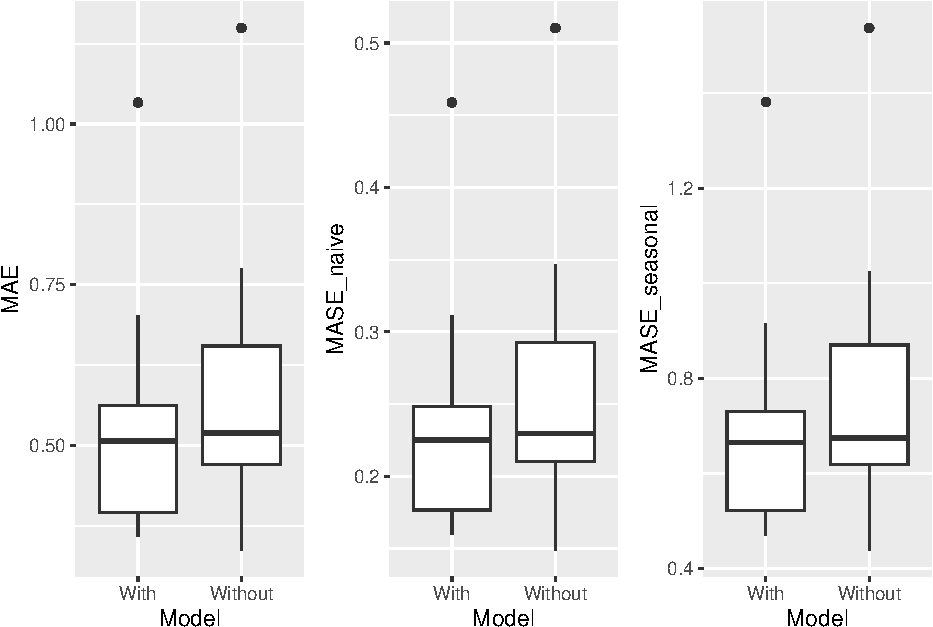
\includegraphics[keepaspectratio]{tempssm_manual_files/tempssm_manual_files/figure-latex/unnamed-chunk-26-1.pdf}}

The tsCV results show that the model with the exogenous variable
performs better than the model without it. The comparison table produced
by \texttt{compare\_ts\_cv()} summarizes the number of folds,
convergence rates, and mean prediction-error metrics for each model,
while the boxplots show how the fold-level errors vary across validation
periods. In this tutorial, the number of tsCV iterations is set to 8 to
reduce execution time. In actual validation, please use a sufficient
number of iterations.

The mean MAE of the model with the exogenous variable is approximately
0.55 °C. Relative to the seasonal amplitude based on monthly mean SST
(about 13.6 °C), this corresponds to roughly 4.0\%. Thus, the prediction
error is small compared with the dominant seasonal scale of variation in
this data set, and may be practically useful for short-term marine
monitoring.

Although the number of validation folds is limited to 8, the model with
the exogenous variable reduces the mean MAE by approximately 9.2\%
compared with the model without the exogenous variable. Similar
improvements are also seen in the MASE metrics. This interpretation
should be kept conditional on the tsCV setting used here, in which
observed PDO values during the test periods are supplied as exogenous
variables.

Taken together, the results consistently support including the PDO index
as an exogenous variable in the state-space model. The PDO coefficient
is statistically significant, indicating a clear effect on temperature
variation. Time-series cross-validation further indicates that this
effect is accompanied by better out-of-sample predictive performance.

These complementary lines of evidence provide robust and multifaceted
support for adopting the exogenous-variable model.

Although this exercise used a single exogenous variable,
\texttt{tempssm()} also supports models with multiple exogenous
variables supplied as multivariate time-series data. Users interested in
broader applications can extend the same workflow to other
environmental, climatic, or ecological covariates. In doing so, model
structure should be considered carefully for the target data, while
checking model diagnostics and out-of-sample predictive performance.

\subsubsection{Comparing Estimation Patterns Between Models With and
Without the Exogenous
Variable}\label{comparing-estimation-patterns-between-models-with-and-without-the-exogenous-variable}

We compare how the estimated patterns of the long-term trend and its
rate of change differ between the models with and without the exogenous
variable.

\begin{Shaded}
\begin{Highlighting}[]
\NormalTok{plt\_level\_without\_ts }\OtherTok{\textless{}{-}} \FunctionTok{autoplot}\NormalTok{(res\_without,}
                                 \AttributeTok{component=}\FunctionTok{c}\NormalTok{(}\StringTok{"level"}\NormalTok{)}
\NormalTok{                                 ) }\SpecialCharTok{+}
  \FunctionTok{labs}\NormalTok{(}\AttributeTok{title=}\StringTok{"Model without the PDO index"}\NormalTok{) }\SpecialCharTok{+}
  \FunctionTok{theme\_classic}\NormalTok{()}

\NormalTok{plt\_drift\_without\_ts }\OtherTok{\textless{}{-}} \FunctionTok{autoplot}\NormalTok{(res\_without, }
                             \AttributeTok{component=}\FunctionTok{c}\NormalTok{(}\StringTok{"drift"}\NormalTok{)}
\NormalTok{                             ) }\SpecialCharTok{+} 
  \FunctionTok{labs}\NormalTok{(}\AttributeTok{title=}\StringTok{"Model without the PDO index"}\NormalTok{) }\SpecialCharTok{+}
  \FunctionTok{theme\_classic}\NormalTok{()}

\NormalTok{plt\_level\_drift\_without\_ts }\OtherTok{\textless{}{-}}\NormalTok{ plt\_level\_without\_ts }\SpecialCharTok{+} 
\NormalTok{  plt\_drift\_without\_ts }\SpecialCharTok{+} 
\NormalTok{  patchwork}\SpecialCharTok{::}\FunctionTok{plot\_layout}\NormalTok{(}\AttributeTok{ncol=}\DecValTok{1}\NormalTok{)}

\FunctionTok{plot}\NormalTok{(plt\_level\_drift\_without\_ts)}
\end{Highlighting}
\end{Shaded}

\pandocbounded{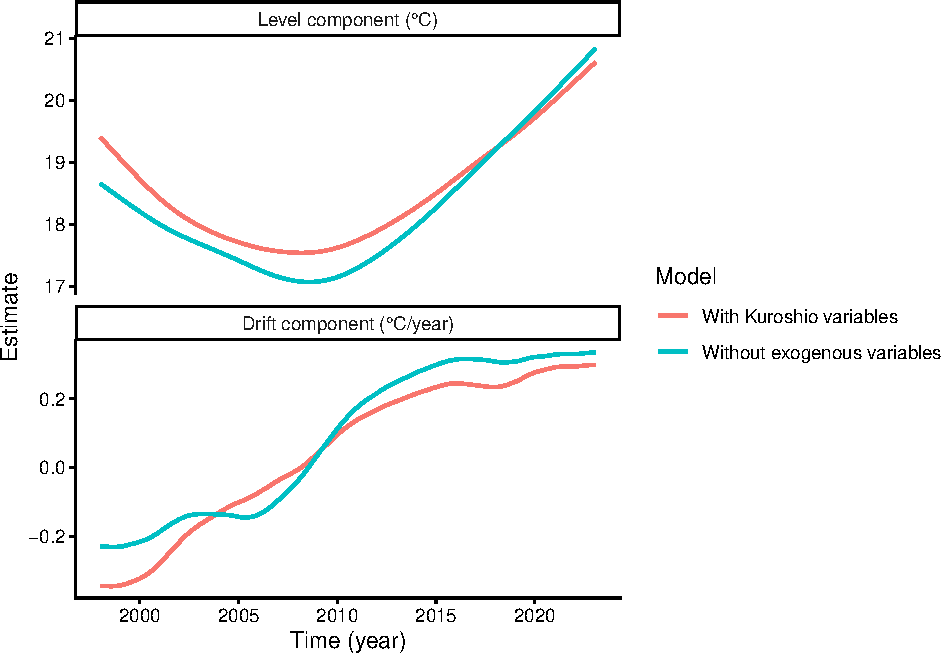
\includegraphics[keepaspectratio]{tempssm_manual_files/tempssm_manual_files/figure-latex/unnamed-chunk-28-1.pdf}}

\begin{Shaded}
\begin{Highlighting}[]
\NormalTok{plt\_level\_with\_ts }\OtherTok{\textless{}{-}} \FunctionTok{autoplot}\NormalTok{(res\_with,}
                          \AttributeTok{component=}\FunctionTok{c}\NormalTok{(}\StringTok{"level"}\NormalTok{)}
\NormalTok{                          )}\SpecialCharTok{+} 
  \FunctionTok{labs}\NormalTok{(}\AttributeTok{title=}\StringTok{"Model with the PDO index"}\NormalTok{) }\SpecialCharTok{+}
  \FunctionTok{theme\_classic}\NormalTok{()}

\NormalTok{plt\_drift\_with\_ts }\OtherTok{\textless{}{-}} \FunctionTok{autoplot}\NormalTok{(res\_with,}
                          \AttributeTok{component=}\FunctionTok{c}\NormalTok{(}\StringTok{"drift"}\NormalTok{)}
\NormalTok{                          ) }\SpecialCharTok{+} 
  \FunctionTok{labs}\NormalTok{(}\AttributeTok{title=}\StringTok{"Model with the PDO index"}\NormalTok{) }\SpecialCharTok{+} 
  \FunctionTok{theme\_classic}\NormalTok{()}

\NormalTok{plt\_level\_drift\_with\_ts }\OtherTok{\textless{}{-}}\NormalTok{ plt\_level\_with\_ts }\SpecialCharTok{+} 
\NormalTok{  plt\_drift\_with\_ts }\SpecialCharTok{+} 
\NormalTok{  patchwork}\SpecialCharTok{::}\FunctionTok{plot\_layout}\NormalTok{(}\AttributeTok{ncol=}\DecValTok{1}\NormalTok{)}

\FunctionTok{plot}\NormalTok{(plt\_level\_drift\_with\_ts)}
\end{Highlighting}
\end{Shaded}

\pandocbounded{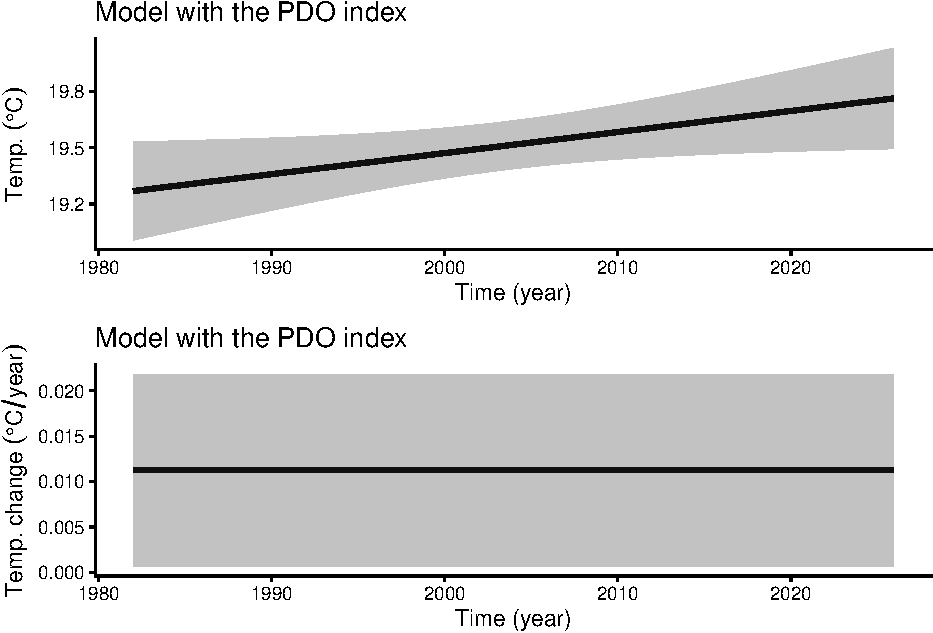
\includegraphics[keepaspectratio]{tempssm_manual_files/tempssm_manual_files/figure-latex/unnamed-chunk-28-2.pdf}}

\begin{Shaded}
\begin{Highlighting}[]
\CommentTok{\#　Smoothing estimate of drift component}
\NormalTok{mean\_drift\_year\_without }\OtherTok{\textless{}{-}} \FunctionTok{get\_drift\_ts}\NormalTok{(res\_without) }\SpecialCharTok{\%\textgreater{}\%}
  \FunctionTok{mean}\NormalTok{()}
\FunctionTok{print}\NormalTok{(mean\_drift\_year\_without)}
\end{Highlighting}
\end{Shaded}

\begin{verbatim}
## [1] 0.03388663
\end{verbatim}

\begin{Shaded}
\begin{Highlighting}[]
\NormalTok{mean\_drift\_year\_with }\OtherTok{\textless{}{-}} \FunctionTok{get\_drift\_ts}\NormalTok{(res\_with) }\SpecialCharTok{\%\textgreater{}\%}
  \FunctionTok{mean}\NormalTok{()}
\FunctionTok{print}\NormalTok{(mean\_drift\_year\_with)}
\end{Highlighting}
\end{Shaded}

\begin{verbatim}
## [1] 0.01124586
\end{verbatim}

The gray areas in the plots above show 95\% confidence intervals.

In the model without an exogenous variable, the plots of the long-term
trend and its rate of change show a wavelike pattern. In contrast, in
the model with the exogenous variable, the long-term trend and its rate
of change show a more stable pattern. This suggests that the wavelike
pattern reflects the influence of the exogenous PDO variable.

The estimated annual rate of SST change over the observation period is
0.0339 in the model without the exogenous variable and 0.0112 in the
model with the exogenous variable.

In this case, the model incorporating the PDO index is considered
preferable for accurately estimating the SST trend. Thus, the SST
warming rate, which was estimated somewhat higher in the model without
the exogenous variable, is estimated more conservatively after
introducing the model with the exogenous variable.

\section{Using Your Own Data}\label{using-your-own-data}

\subsection{Quick Example}\label{quick-example}

\texttt{my\_ts} is a user-supplied \texttt{ts} object containing
temperature time-series data. It can be passed directly to
\texttt{tempssm()}.

\begin{Shaded}
\begin{Highlighting}[]
\DocumentationTok{\#\# example of ts object (not run)}
\DocumentationTok{\#\# my\_ts \textless{}{-} ts(rnorm(100), frequency = 12)}
\NormalTok{res }\OtherTok{\textless{}{-}} \FunctionTok{tempssm}\NormalTok{(my\_ts)}
\end{Highlighting}
\end{Shaded}

\subsection{Preparing Your Own
Dataset}\label{preparing-your-own-dataset}

\subsubsection{CSV Format}\label{csv-format}

Prepare a CSV file of monthly temperature time series with the following
columns: - Year - Month - Temp

Example:

\begin{Shaded}
\begin{Highlighting}[]
\NormalTok{Year,Month,Temp}
\NormalTok{2010,8,13.6}
\NormalTok{2010,9,6.8}
\NormalTok{2010,10,NA}
\NormalTok{2010,11,{-}1.4}
\NormalTok{...}
\end{Highlighting}
\end{Shaded}

\begin{itemize}
\tightlist
\item
  Use NA for missing temperature values, and always keep the
  corresponding Year and Month entries.
\item
  The CSV file must be comma-separated and UTF-8 encoded.
\end{itemize}

\subsubsection{Converting CSV to a Time
Series}\label{converting-csv-to-a-time-series}

An example CSV file included in this package is available in
inst/extdata. The example dataset contains monthly air temperature
observations from Mt. Akadake, Hokkaido, Japan (1,840 m). The original
data are available from the Monitoring Sites 1000 Project of the
Ministry of the Environment of Japan (KOZ01.zip,
\url{https://www.biodic.go.jp/moni1000/findings/data/index.html}).

\begin{Shaded}
\begin{Highlighting}[]
\NormalTok{path }\OtherTok{\textless{}{-}} \FunctionTok{system.file}\NormalTok{(}\StringTok{"extdata"}\NormalTok{, }\StringTok{"example\_monthly\_temp.csv"}\NormalTok{, }\AttributeTok{package =} \StringTok{"tempssm"}\NormalTok{)}
\NormalTok{akadake\_temp }\OtherTok{\textless{}{-}}\NormalTok{ tempssm}\SpecialCharTok{::}\FunctionTok{read\_monthly\_temp\_ts}\NormalTok{(path)}
\FunctionTok{head}\NormalTok{(akadake\_temp)}
\end{Highlighting}
\end{Shaded}

\begin{verbatim}
##        Jan Feb Mar Apr May Jun Jul   Aug   Sep   Oct   Nov   Dec
## 2010                                13.6   6.8   0.2  -6.8 -12.5
## 2011 -18.8
\end{verbatim}

The \texttt{read\_monthly\_temp\_ts()} function reads this type of CSV
file and converts it into an R \texttt{ts} object for use with
\texttt{tempssm()}. If finer control is needed, you can also construct a
\texttt{ts} object manually; see the \texttt{stats::ts} documentation
for details:
\url{https://search.r-project.org/R/refmans/stats/html/ts.html}.

\section{References}\label{references}

The statistical modeling framework implemented in \texttt{tempssm} is
based on the methodology described in Baba et al.~(2024), and the
accompanying supplementary materials and code repository served as the
initial source for development of this package.

Baba, S., Ishii, H., and Yoshiyama, T. (2024). Estimating sea
temperature trends using a linear Gaussian state-space model in
Jogashima, Kanagawa, Japan. \emph{Bulletin of the Japanese Society of
Fisheries Oceanography}, 88(3), 190--199. (In Japanese with an English
abstract.) \url{https://doi.org/10.34423/jsfo.88.3_190}

Baba, S. (2024). Supplementary code and test data for estimating sea
temperature trends using a linear Gaussian state-space model. GitHub
repository:
\url{https://github.com/logics-of-blue/sea-temperature-trend-jogashima}

Helske, J. (2017). KFAS: Exponential Family State Space Models in R.
\emph{Journal of Statistical Software}, 78(10), 1--39.
\url{https://doi.org/10.18637/jss.v078.i10}

\section{Appendix: Utility Functions}\label{appendix-utility-functions}

The following utility functions are provided to support data preparation
and exploratory analysis.

\subsection{\texorpdfstring{1.
\texttt{read\_monthly\_temp\_ts()}}{1. read\_monthly\_temp\_ts()}}\label{read_monthly_temp_ts}

The \texttt{read\_monthly\_temp\_ts()} function converts monthly
temperature data stored in a CSV file into an R \texttt{ts} object. By
enforcing a simple and consistent data format, it is intended to make
externally prepared time-series data easier to import into tempssm.

\subsubsection{Example}\label{example}

For monthly temperature data, prepare a CSV file with a header row. By
default, the column names must be \texttt{Year}, \texttt{Month}, and
\texttt{Temp}, where \texttt{Temp} represents the observed temperature
value.

\begin{Shaded}
\begin{Highlighting}[]
\NormalTok{Year,Month,Temp}
\NormalTok{2001,1,10.4}
\NormalTok{2001,2,8.2}
\NormalTok{2001,3,NA}
\NormalTok{2001,4,13.6}
\NormalTok{2001,5,16.1}
\NormalTok{...}
\end{Highlighting}
\end{Shaded}

\begin{itemize}
\tightlist
\item
  Use NA for missing temperature values, and always keep the
  corresponding Year and Month entries.
\item
  The CSV file must be comma-separated and UTF-8 encoded.
\end{itemize}

The following example uses the sample CSV file included in the package.
It contains monthly air temperature observations from Mt. Akadake,
Hokkaido, Japan.

\begin{Shaded}
\begin{Highlighting}[]
\NormalTok{path }\OtherTok{\textless{}{-}} \FunctionTok{system.file}\NormalTok{(}\StringTok{"extdata"}\NormalTok{, }\StringTok{"example\_monthly\_temp.csv"}\NormalTok{, }\AttributeTok{package =} \StringTok{"tempssm"}\NormalTok{)}

\CommentTok{\# Read the CSV file and convert it to a monthly ts object}
\NormalTok{temp\_ts }\OtherTok{\textless{}{-}} \FunctionTok{read\_monthly\_temp\_ts}\NormalTok{(path)}
\FunctionTok{head}\NormalTok{(temp\_ts)}
\end{Highlighting}
\end{Shaded}

\begin{verbatim}
##        Jan Feb Mar Apr May Jun Jul   Aug   Sep   Oct   Nov   Dec
## 2010                                13.6   6.8   0.2  -6.8 -12.5
## 2011 -18.8
\end{verbatim}

\subsection{\texorpdfstring{2.
\texttt{convert\_monthly\_df\_to\_ts()}}{2. convert\_monthly\_df\_to\_ts()}}\label{convert_monthly_df_to_ts}

The \texttt{convert\_monthly\_df\_to\_ts()} function converts a data
frame containing monthly temperature data into an R \texttt{ts} object.
It is designed to support workflows in which temperature data are first
imported or prepared as a data frame and then used for time-series
analysis.

The input data frame is expected to contain at least two columns: a date
column (\texttt{Date}) and a temperature column (\texttt{Temp}). For the
date column (\texttt{Date}), assign an arbitrary day of the month, such
as the first day, so that the dates correspond to monthly aggregated
temperature values.

\subsubsection{Example}\label{example-1}

\begin{Shaded}
\begin{Highlighting}[]
\CommentTok{\# Create a data frame of monthly temperature data}
\NormalTok{df }\OtherTok{\textless{}{-}} \FunctionTok{data.frame}\NormalTok{(}
  \AttributeTok{Date =} \FunctionTok{as.Date}\NormalTok{(}\FunctionTok{c}\NormalTok{(}
    \StringTok{"2001{-}01{-}01"}\NormalTok{,}
    \StringTok{"2001{-}02{-}01"}\NormalTok{,}
    \StringTok{"2001{-}03{-}01"}\NormalTok{,}
    \StringTok{"2001{-}04{-}01"}\NormalTok{,}
    \StringTok{"2001{-}05{-}01"}\NormalTok{)}
\NormalTok{    ),}
  \AttributeTok{Temp =} \FunctionTok{c}\NormalTok{(}\FloatTok{10.4}\NormalTok{, }\FloatTok{8.2}\NormalTok{, }\ConstantTok{NA}\NormalTok{, }\FloatTok{13.6}\NormalTok{, }\FloatTok{16.1}\NormalTok{)}
\NormalTok{  )}

\CommentTok{\# Convert to a monthly ts object}
\NormalTok{temp\_ts }\OtherTok{\textless{}{-}} \FunctionTok{convert\_monthly\_df\_to\_ts}\NormalTok{(df)}
\FunctionTok{head}\NormalTok{(temp\_ts)}
\end{Highlighting}
\end{Shaded}

\begin{verbatim}
##       Jan  Feb  Mar  Apr  May
## 2001 10.4  8.2   NA 13.6 16.1
\end{verbatim}

\subsection{\texorpdfstring{3.
\texttt{get\_jma\_sst\_ts()}}{3. get\_jma\_sst\_ts()}}\label{get_jma_sst_ts}

The \texttt{get\_jma\_sst\_ts()} function downloads daily mean sea
surface temperature (SST) data for Japanese coastal waters provided by
the Japan Meteorological Agency (JMA). It aggregates the daily values
into monthly means and returns the resulting time series as an object of
class \texttt{ts}.

\subsubsection{Example}\label{example-2}

The following example demonstrates how to download SST data for the
southern coastal waters of Ibaraki Prefecture, Japan.

The argument \texttt{sea\_area\_id} specifies the numeric identifier of
a sea area defined by JMA. For example, \texttt{138} corresponds to the
coastal waters off southern Ibaraki. A list of available sea area IDs
and their corresponding regions is provided by JMA at:

\url{https://www.data.jma.go.jp/kaiyou/data/db/kaikyo/series/engan/eg_areano.html}

\begin{Shaded}
\begin{Highlighting}[]
\NormalTok{sst\_138\_ts }\OtherTok{\textless{}{-}} \FunctionTok{get\_jma\_sst\_ts}\NormalTok{(}\AttributeTok{sea\_area\_id =} \DecValTok{138}\NormalTok{)}
\FunctionTok{head}\NormalTok{(sst\_138\_ts)}
\end{Highlighting}
\end{Shaded}

\begin{verbatim}
##           Jan      Feb      Mar      Apr      May      Jun
## 1982 15.04419 14.22500 13.63903 15.31933 17.52258 19.52300
\end{verbatim}

\subsection{\texorpdfstring{4.
\texttt{compute\_temp\_anomaly()}}{4. compute\_temp\_anomaly()}}\label{compute_temp_anomaly}

The \texttt{compute\_temp\_anomaly()} function computes anomalies from a
time series provided as an R \texttt{ts} object. Anomalies are
calculated by subtracting the corresponding long-term mean for each
periodic unit, such as month, from each observation. This transformation
is useful for examining interannual variability after removing periodic
effects.

The reference period used to compute anomalies can be specified via a
function argument. By default, the climatology is computed over the
entire available time series (see \texttt{?compute\_temp\_anomaly}).

This transformation is useful for exploratory analysis and modeling
applications that focus on departures from typical seasonal conditions.

\subsubsection{Example}\label{example-3}

\begin{Shaded}
\begin{Highlighting}[]
\CommentTok{\# Generate temperature anomalies}
\FunctionTok{data}\NormalTok{(niigata\_sst)}
\NormalTok{niigata\_sst\_anomaly }\OtherTok{\textless{}{-}} \FunctionTok{compute\_temp\_anomaly}\NormalTok{(niigata\_sst)}
\NormalTok{plt\_niigata\_sst\_anomaly }\OtherTok{\textless{}{-}}\NormalTok{ forecast}\SpecialCharTok{::}\FunctionTok{autoplot}\NormalTok{(niigata\_sst\_anomaly) }\SpecialCharTok{+}
  \FunctionTok{labs}\NormalTok{(}\AttributeTok{y =} \FunctionTok{expression}\NormalTok{(Temp.}\SpecialCharTok{\textasciitilde{}}\NormalTok{(degree}\SpecialCharTok{*}\NormalTok{C)), }
       \AttributeTok{x =} \StringTok{"Time (year)"}\NormalTok{)}
\FunctionTok{plot}\NormalTok{(plt\_niigata\_sst\_anomaly) }
\end{Highlighting}
\end{Shaded}

\pandocbounded{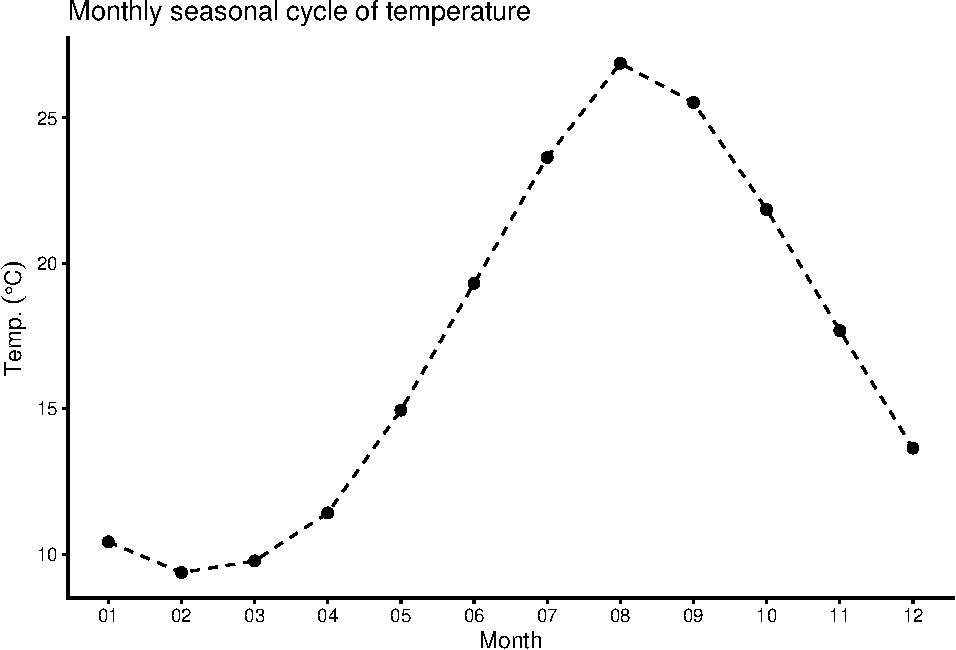
\includegraphics[keepaspectratio]{tempssm_manual_files/tempssm_manual_files/figure-latex/unnamed-chunk-34-1.pdf}}

\subsection{\texorpdfstring{5.
\texttt{compute\_monthly\_climatology()}}{5. compute\_monthly\_climatology()}}\label{compute_monthly_climatology}

The \texttt{compute\_monthly\_climatology()} function computes the
climatological mean seasonal cycle from a \texttt{ts} object by
averaging each seasonal value across years. It is primarily intended for
exploratory analysis and visualization of seasonal structure in
temperature time series.

\subsubsection{Example}\label{example-4}

\begin{Shaded}
\begin{Highlighting}[]
\FunctionTok{data}\NormalTok{(niigata\_sst)}
\NormalTok{monthly\_seasonal\_cycle\_niigata\_sst }\OtherTok{\textless{}{-}} \FunctionTok{compute\_monthly\_climatology}\NormalTok{(niigata\_sst) }
\FunctionTok{summary}\NormalTok{(monthly\_seasonal\_cycle\_niigata\_sst)}
\end{Highlighting}
\end{Shaded}

\begin{verbatim}
##      Month        Temperature    
##  Min.   : 1.00   Min.   : 9.365  
##  1st Qu.: 3.75   1st Qu.:11.169  
##  Median : 6.50   Median :16.318  
##  Mean   : 6.50   Mean   :17.036  
##  3rd Qu.: 9.25   3rd Qu.:22.294  
##  Max.   :12.00   Max.   :26.873
\end{verbatim}

\begin{Shaded}
\begin{Highlighting}[]
\NormalTok{plt\_monthly\_seasonal\_cycle\_niigata\_sst }\OtherTok{\textless{}{-}} \FunctionTok{ggplot}\NormalTok{(}
  \AttributeTok{data =}\NormalTok{ monthly\_seasonal\_cycle\_niigata\_sst,}
  \FunctionTok{aes}\NormalTok{(}\AttributeTok{x =}\NormalTok{ Month, }\AttributeTok{y =}\NormalTok{ Temperature)}
\NormalTok{) }\SpecialCharTok{+}
  \FunctionTok{geom\_point}\NormalTok{(}\AttributeTok{size =} \DecValTok{2}\NormalTok{) }\SpecialCharTok{+}
  \FunctionTok{geom\_line}\NormalTok{(}\AttributeTok{linetype =} \StringTok{"dashed"}\NormalTok{) }\SpecialCharTok{+}
  \FunctionTok{labs}\NormalTok{(}
    \AttributeTok{title =} \StringTok{"Monthly seasonal cycle of temperature"}\NormalTok{,}
    \AttributeTok{x =} \StringTok{"Month"}\NormalTok{,}
    \AttributeTok{y =} \FunctionTok{expression}\NormalTok{(Temp.}\SpecialCharTok{\textasciitilde{}}\NormalTok{(degree}\SpecialCharTok{*}\NormalTok{C))}
\NormalTok{  ) }\SpecialCharTok{+}
  \FunctionTok{scale\_x\_continuous}\NormalTok{(}
    \AttributeTok{breaks =} \DecValTok{1}\SpecialCharTok{:}\DecValTok{12}\NormalTok{,}
    \AttributeTok{labels =} \FunctionTok{sprintf}\NormalTok{(}\StringTok{"\%02d"}\NormalTok{, }\DecValTok{1}\SpecialCharTok{:}\DecValTok{12}\NormalTok{)}
\NormalTok{  ) }\SpecialCharTok{+}
  \FunctionTok{theme\_classic}\NormalTok{()}


\FunctionTok{plot}\NormalTok{(plt\_monthly\_seasonal\_cycle\_niigata\_sst)}
\end{Highlighting}
\end{Shaded}

\pandocbounded{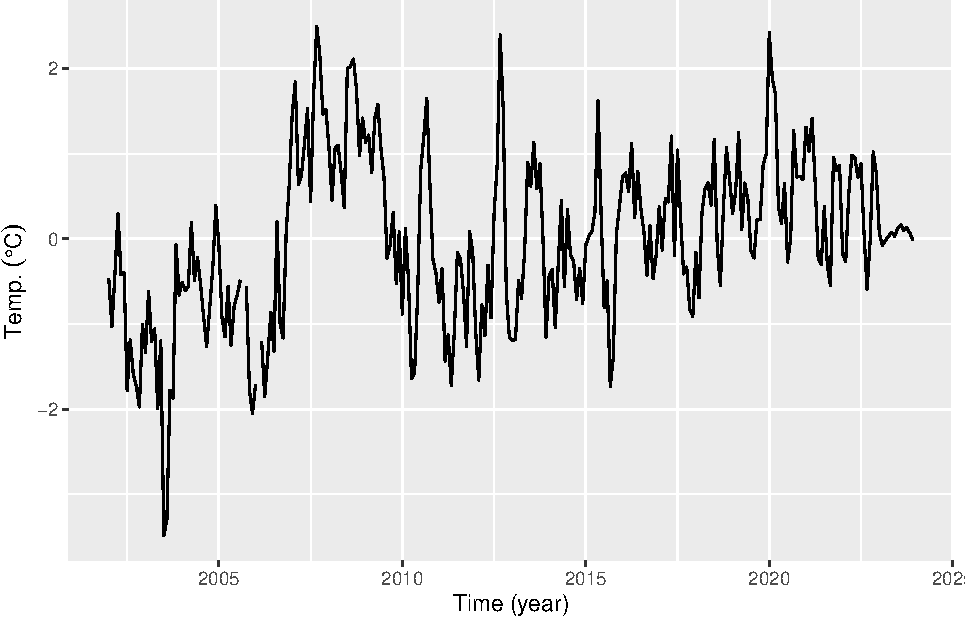
\includegraphics[keepaspectratio]{tempssm_manual_files/tempssm_manual_files/figure-latex/unnamed-chunk-35-1.pdf}}

\end{document}
